\documentclass[12pt,a4paper]{article}
\usepackage[latin1]{inputenc}
\usepackage{float}
\usepackage{amsmath}
\usepackage{amsfonts}
\usepackage{amssymb}
\usepackage{graphicx}
\usepackage[hidelinks]{hyperref}
\usepackage{changepage}
\usepackage{subfig}
\usepackage{placeins}



\author{Davide Cocco - 944122\\
	Marco Gasperini - 944922}
\date{A.Y. 2019/2020 - Prof. Di Nitto Elisabetta}


\title{
	\textbf{\Huge{SafeStreets}} \\
	\large Design Document
}

\begin {document}

	\begin{figure}
		\centering
		
\includegraphics[width=1.0\linewidth]{Images/polimi.jpg}
	\end{figure}

	\maketitle
	\newpage
	\tableofcontents
	\newpage

\section{INTRODUCTION}
\subsection{Purpose}
This \texttt{Design Document (DD)} for the SafeStreets software will provide a functional description of the system by describing its architecture. 
It will eventually be used by the development team as a blueprint to guide the engineering of the application.
\subsection{Scope}
The main objective of the S2B will be assisting (thus not substituting) authorities and officers in handling traffic violations though a crowd-sourced platform in which civilians can participate. 
A mobile application will allow users, both civilians and officers, to report violations through the use of the camera and the GPS, sending the data to authorities who will process such reports. 
Law enforcement will be aided by a data mining system which will produce relevant data about the registered violations, and the S2B will be able to automatically compile a ticket and send it to
the municipality's VLA as soon as an officer personally convalidates a violation.
\subsection{Definitions, Acronyms, Abbreviations}
\subsubsection{Definitions}
\begin{itemize}
\item \texttt{Violation | Offence:} we will strictly refer to any kind of static traffic violation, especially parking violations. 
\item \texttt{Authority:} a law enforcement authority which is manages traffic violations, it could be the local police, the traffic wardens etc. We will refer with this term also to the personnel which operates the web application in the authorities' headquarters.
\item \texttt{User:} refers to the users of the mobile application, that is officers and civilians.
\end{itemize}
\subsubsection{Acronyms}
\begin{itemize}
\item \texttt{S2B:} software to be.
\item \texttt{RASD:} Requirement Analysis and Specification Document.
\item \texttt{HFVZ:} high violation frequency zone.
\item \texttt{GPS:} Global Positioning System.
\item \texttt{GDPR:} General Data Protection Regulation.
\item \texttt{DW:} data warehouse.
\item \texttt{VLA:} Vehicle Licensing Authority.
\item \texttt{RACS:} Reliable Array of Cloned Services.
\item \texttt{RAPS:} Reliable Array of Partitioned Services.
\item \texttt{GUI:} Graphical User Interface.
\item \texttt{DMZ:} Demilitarized zone.
\item \texttt{ADS:} Application and Data server of the authorities.
\item \texttt{API:} Application Programming Interface.
\item \texttt{OS:} Operative System.
\item \texttt{MVP:} Minimum Viable Product.
\end{itemize}
\subsubsection{Abbreviations}
\begin{itemize}
	\item {[Gn]}: n-goal.
	\item {[Rn]}: n-requirement.
	\item {[Dn]}: n-domain assumption
	\item {App}: application.
\end{itemize}
\subsection{Revision History}
\subsection{Reference Documents}
\subsection{Document Structure}
\begin{itemize}
\item \textbf{Introduction}: includes the purpose and scope of the document along with some relevant definitions and acronyms used throughout the document.
\item \textbf{Architectural design}: this section is focused on the main components used for this system and the relationships between them, providing information about their
deployment and how they operate. it also focuses on the architectural styles and the design patterns adopted for designing the system.
\item \textbf{User interface design}: this section provides an overview on how the User Interface will work with UX diagrams.
\item \textbf{Requirements traceability}: in this sections the requirements highlighted in the RASD document will be associated with the design elements explained in this document.
\item \textbf{Implementation, integration and test plan}: in this section we identify the order in which we plan to implement, test and integrate the subcomponents of the system.
\end{itemize}
\newpage
\section{ARCHITECTURAL DESIGN}
\subsection{High level overview}
			\begin{figure}[H]
				\centering
					\begin{adjustwidth}{-25mm}{-25mm}
					        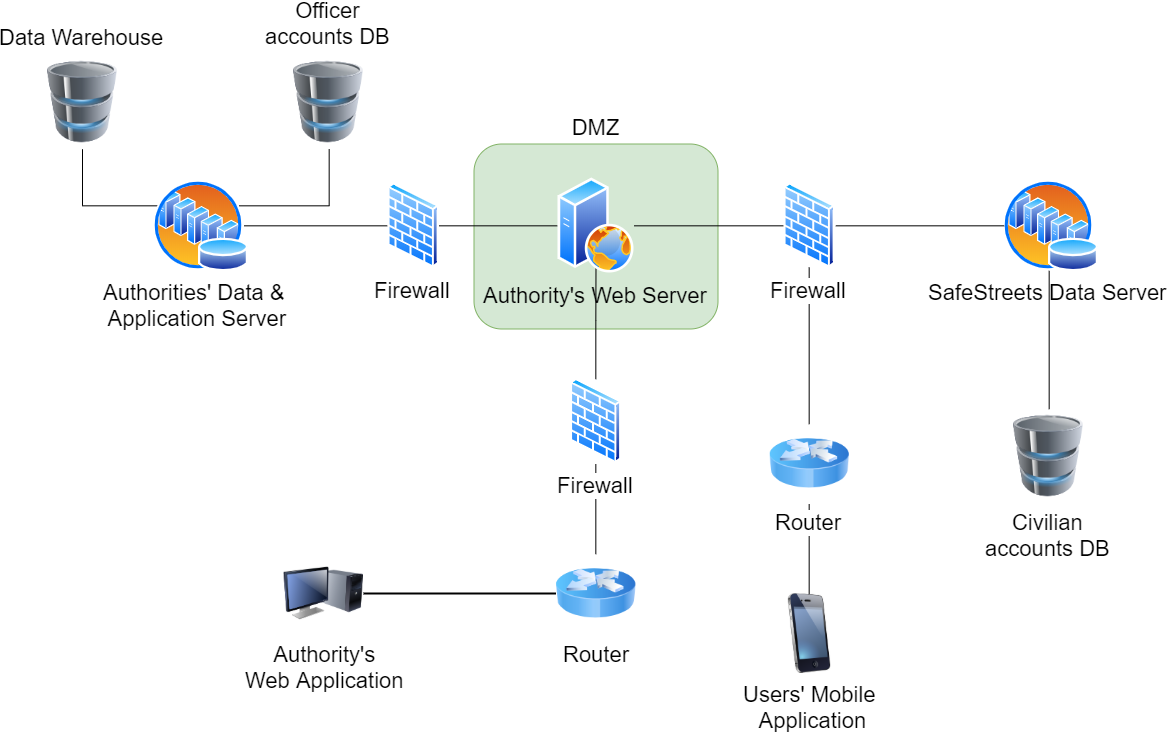
\includegraphics[width=.9\paperwidth,keepaspectratio]{Images/highlevel}
					\end{adjustwidth}
				\caption{High Level Structure with a single Authority and a single User}
			\end{figure}
The three logical layers of the S2B are distributed in a \textbf{three-tier architecture}:
\begin{itemize}
\item \textbf{Presentation layer:} two hard clients:
\begin{itemize}
\item the GUI at the authority's web application is the tool thanks to which the authority's personnel can add officers, receive reports from the users through HTTP calls thanks to a REST architecture embedded in the web server, and validate or invalidate them. It can thus interact directly with the web server, and rarely with the SafeStreets' server to which it sends ban requests. The web server is isolated from the outside by firewalls for increased security and to protect the ADS even if the web server is compromised. The only logic that will be implemented directly at the this client will be the supervised algorithm to recognize plates: this way we can reduce latency, because since the overhead to effectively send a correct plate frame will be pretty heavy, we remove the step to contact the application server and instead execute this function directly at the authorities' location. Anything else will be handled as notifications forwarded to the ADS to limit the computational power used at the authorities' locations.
\item the GUI at the mobile application, which can be used to file reports and send them to the Authority's web server by all users, and which allows officers to check reports and sign automated tickets (and also receives slightly different updates which
include sensitive data to be made unreadable by civilians). 
\end{itemize}
Moreover, both clients must be able to "unpack" the received updates' representations into a format understandable to the user.
\item \textbf{Application layer:} the hypermedia at the mobile application moves from a state to another thanks to the updates received by the authorities' web servers (which are themselves sent to the authorities by the ADS, and then are periodically spread to the clients in the network). While the web server constitutes an interface protected by a DMZ which clients are forced to invoke when applicative functions are needed, the ADS hosts the update producing and ticket emission functionalities. It is important to denote the fact that since every Authority owns a web server, calls received from the mobile units can be handled by any of the authorities for load balancing.  Thus we can say that both the Web server located at the authorities' location and the applicative functions of the ADS constitute this layer. 
\item \textbf{Data layer:} three instances where data access is needed:
\begin{itemize}
\item for managing the civilian accounts and bans, at the SafeStreets server;
\item for managing the officer accounts, at the ADS;
\item for reading and writing historical data about reports in the data warehouse, again at the ADS;
Therefore we can say that application and data services are "partially merged" as the ADS hosts both an application and a data server.
\end{itemize}
\end{itemize}

It is important to notice how the ADS could be implemented in a \texttt{RAPS architecture} where multiple ADS each own a single microservice, for example a server could handle ticket emission, another one officer accounts, and another one update mining and spreading. Another configuration could be assigning an ADS for each authority. 
Web Servers are installed at the authority's location, one for each authority, to better serve nearby mobile units and balance loads, especially in big cities.
The SafeStreet servers could be arranged in a \texttt{RACS architecture} to handle requests from great numbers of civilians.
In some settings such as small towns a lightweight version of the architecture could be employed by running the web server directly in the same machine where the Authority's client is running instead of a standalone device, thus making it a two-tier architecture since the web server wouldn't be separed from the presentation layer anymore.


\newpage
\subsection{Component view}
\subsubsection{High Level Component Diagram}
The following diagrams illustrate the system components and the interfaces through which they interact to fullfil their functionalities. The diagram is focused on the application tier, so the remaining tiers (the presentation tier and the data tier) are shown as black-box.
First we highlight a distinction between Client side and Server side:
\begin{itemize}
\item The Client side is composed by two components, \textit{Web Application} and \textit{Mobile Application}. The first is referred to the Authorities client, latter to the User client (Civilian and Officer).
\item The Server side is composed of three main components: \textit{Authorities Web Services} manages the authorities client, through the \textit{AuthoritiesWebServices} interface server-side; the other two services are the \textit{Civilian Mobile Services} and the \textit{Officer Mobile Services} that manage  the \textit{Mobile Application} from two distinct interfaces.
\end{itemize}
\begin{figure}[H]
		\centering
			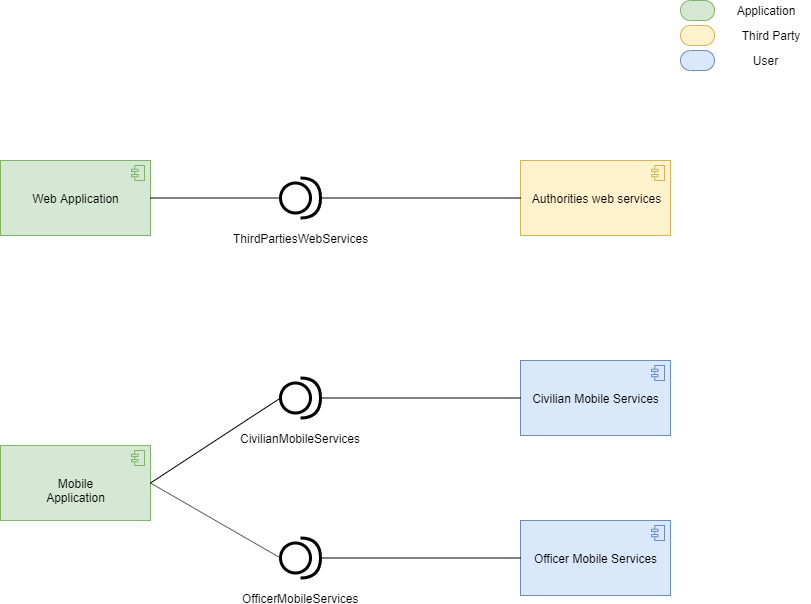
\includegraphics[width=1.0\linewidth]{Images/ComponentDiagram}
		\caption{Component diagram}
\end{figure}

\subsubsection{Civilian Mobile Services Projection}
Civilian Mobile Services subsystem is made of four components: Report Module, Update Module, Data Manager Module and Civilian Authentication Module.
These components provide the Mobile Application the following interfaces: ReportHandler, UpdateHandler, DataManager and CivilianAuthenticationHandler. The Modules also communicate with the map, gps and email services, in the end with a DBMS; the first one allows to collect the mined data about reports in the data warehouse, the latter manages user accesses of any form.
\begin{figure}[H]
				\centering
					\begin{adjustwidth}{-25mm}{-25mm}
					        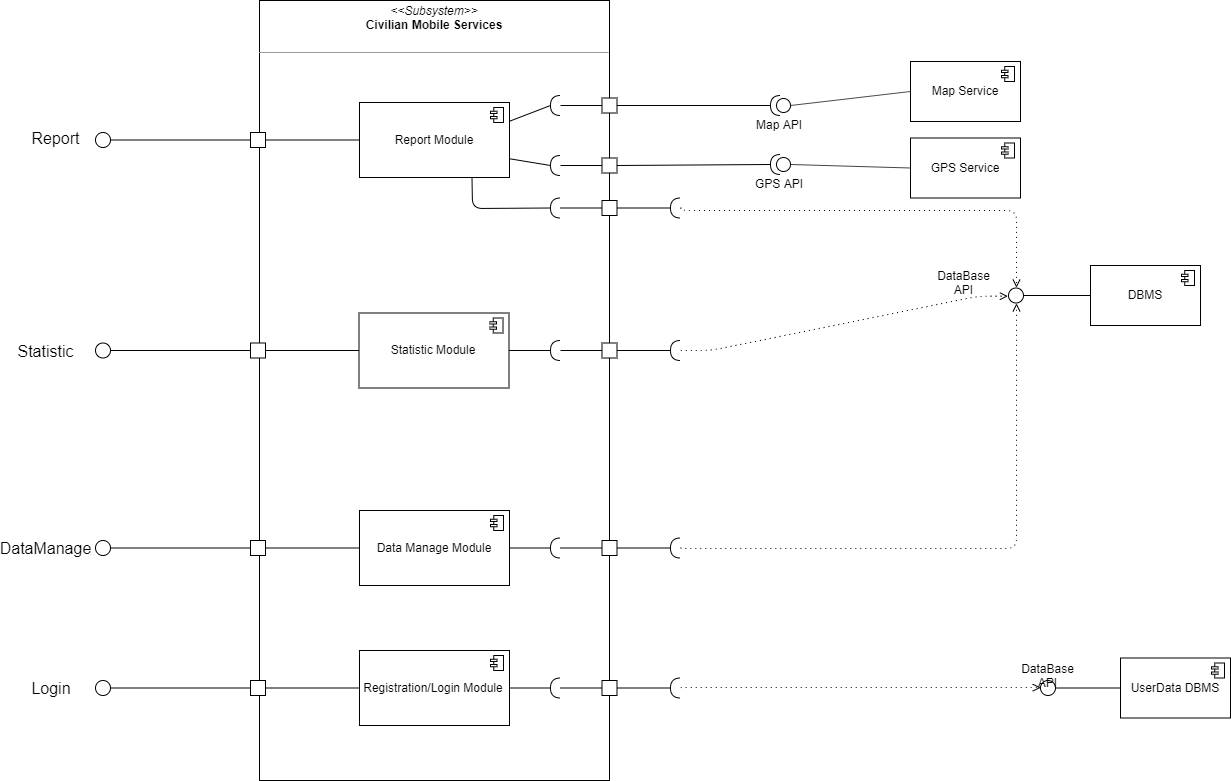
\includegraphics[width=0.9\paperwidth]{Images/CivilianMobileServicesProjection}
					\end{adjustwidth}
			\end{figure}
\newpage
\textbf{Module Functionalities}
\begin{itemize}
	\item \texttt{Report Module}: this module manages the reports done by Civilians and their sending to the Authority's Web server. It will allow the user to take photos of the violation, enter a description of it, timestamp it and attach geolocation coordinates thanks to the GPS API, and also handle all the communication needed for the plate recognition algorithm to work.
	\item \texttt{Update Module}: this module handles the receiving and visualizing of the mined data, among them info about HFVZs, through the Map API.
	\item \texttt{Data Manager Module}: this module allows civilians to manage their personal data (for instance changing their e-mail address or password).
	\item \texttt{Civilian Authentication Module}: this module handles the registration and login requests by civilians, and thus providing the effects of an eventual ban.
\end{itemize}
\newpage
\subsubsection{Officer Mobile Services Projection}
Officer Mobile Services subsystem is an enriched version of the civilian one to accomodate the advanced functions accessible to officers. It is made of four components: Report Module, Update Module, Check Report Module and Officer Authentication Module.
The Report Module works in the same way as the civilian mobile services, while the Update Module possesses quite a few different features to assist the officer. The Check Report Module manages the practice of checking violations by the officer
which might eventually result in a ticket being compiled. The Officer Authentication Module communicates with the Authorities Web Server and not with the SafeStreets server because officer data is kept in the ADS. 
\begin{figure}[H]
				\centering
					\begin{adjustwidth}{-25mm}{-25mm}
					        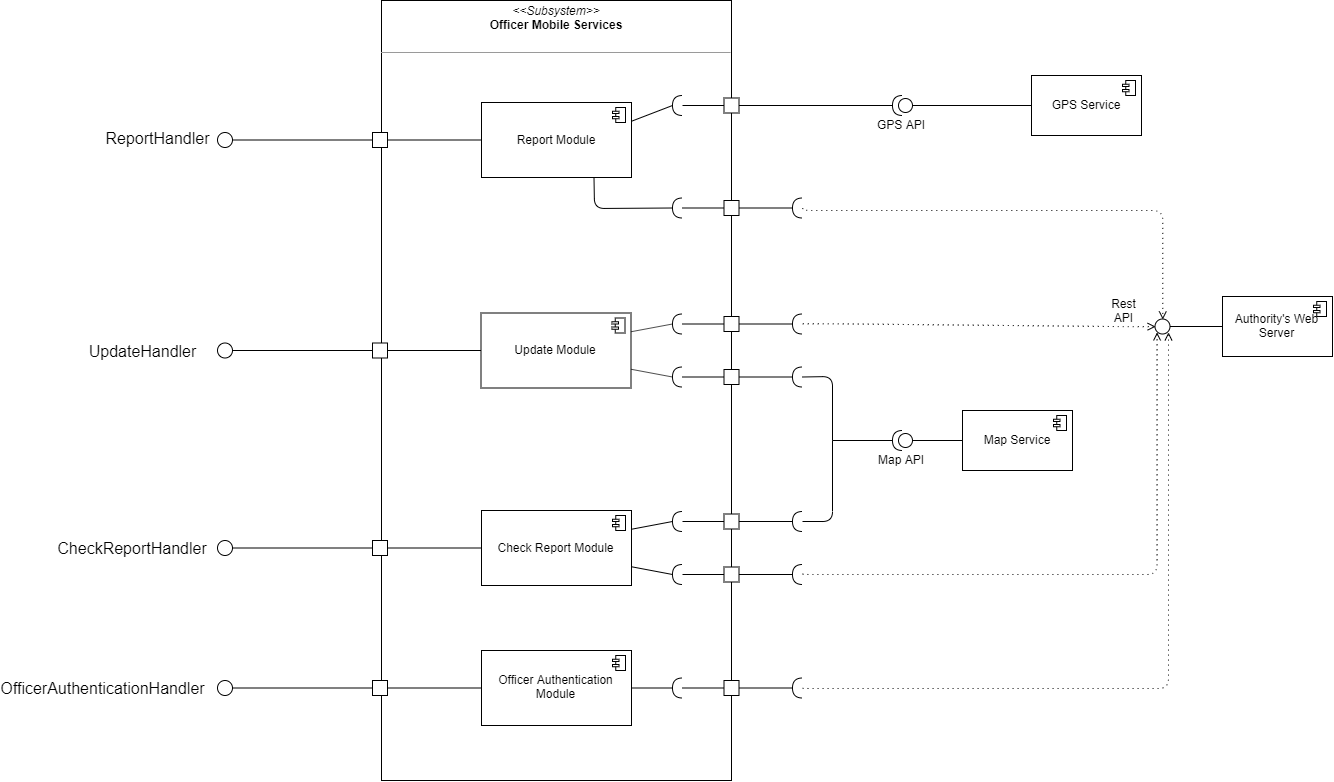
\includegraphics[width=0.9\paperwidth]{Images/OfficerMobileServicesProjection}
					\end{adjustwidth}
			\end{figure}
\newpage
\textbf{Module Functionalities}
\begin{itemize}
	\item \texttt{Report Module}: works in the same way as the Civilian's one, as officers will also be able to report violations.
	\item \texttt{Update Module}: just as the Civilian's one, but enriched with more updates that should only be accessible to law enforcement agents, such as the most egregious offenders list, newly added reports to the map, etc.
	\item \texttt{Check Report Module}: this module allows the officers to confirm the presence of a violation (and the correctness of the plate shown in the report) and enter a secret PIN to allow the emission of a ticket.
	\item \texttt{Officer Authentication Module}: this module handles the registration and login requests by officers.

\end{itemize}
\newpage
\subsubsection{Authorities Web Services Projection}
The Authorities Web Services are carried out by the Web Server and the ADS, which implements most functions of the application. Five Modules will be implemented to fulfill every functionality: Validation Report, Authority Update, Officer Registration, Officer Authentication, Ticket Emission. Web Server and ADS are strongly intertwined to provide the functionalities which all the three actors' clients need: the web server is in fact an interface which provides a layer for communication for the clients to interact with the ADS, for enhanced security, as every HTTP call which eventually has to reach the ADS to execute some logic has to pass through the web server at some authority's location.
\begin{figure}[H]
				\centering
					\begin{adjustwidth}{-25mm}{-25mm}
					        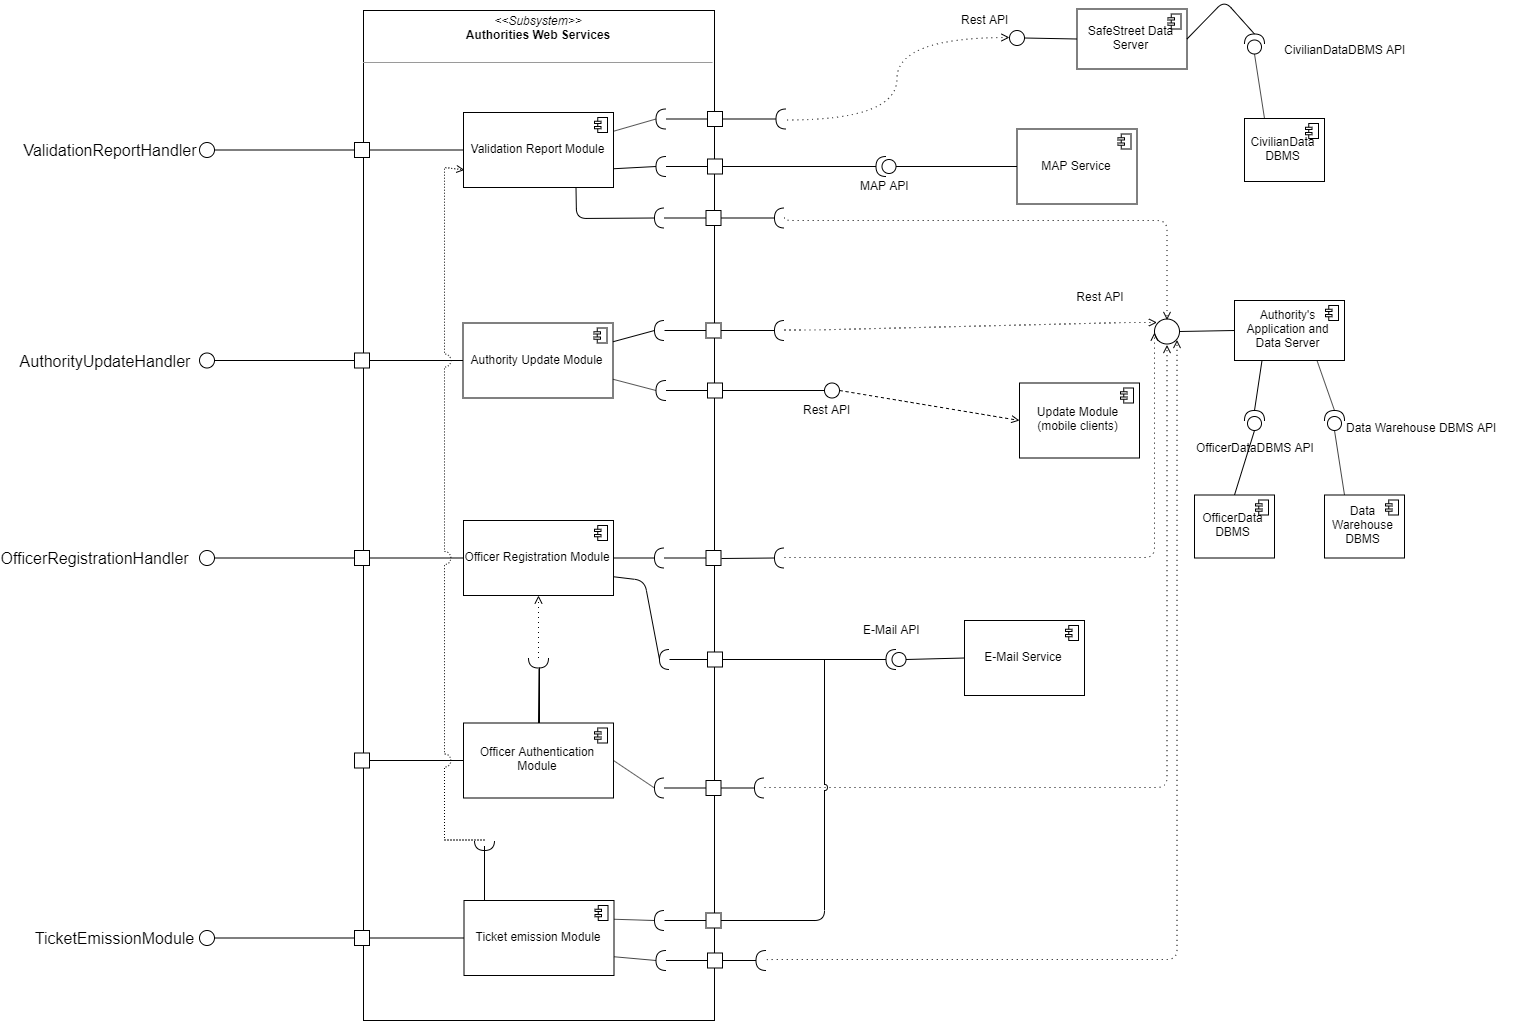
\includegraphics[width=0.9\paperwidth]{Images/AuthoritiesServicesProjection}
					\end{adjustwidth}
			\end{figure}
\newpage
\textbf{Module Functionalities}
\begin{itemize}
	\item \texttt{Validation Report Module}: this module handles the functionality for validating reports by the authority's personnel and the subsequent adding to the DW.  Also the issuing of bans which is performable while invalidating reports.
	\item \texttt{Authority Update Module}: this module not only handles the receiving of updates by the ADS at the web server location (the updates are the same received by the officers, plus the list of currently active officers), but also the mining which will be run in the ADS by periodically querying the DW to retrieve the data which will be packed to form the updates, that will be sent to the web servers and spread by them to the mobile units.
	\item \texttt{Officer Registration Module}: allows the authority to add new officers, communicating the addition both to the officer via mail and to the ADS. Also manages the first insertion of the secret pin by the officer.
	\item \texttt{Officer Authentication Module}: this module authenticates the officers' login requests from the Officer Authentication Module of the Officer Services, and the pin insertion from the Check Report module.
	\item \texttt{Officer Authentication Module}: this module compliles the automated tickets with the signature of the officers and data about the report, and sends it to the VLA via mail.
\end{itemize}
\newpage
\subsubsection{Complete Component Diagram}
This diagram shows the interactions between all the subsystems of the application for better clarity. The presence of multiple REST APIs instead of a single comprehensive one has been modeled to show the different connections between modules without ambiguity. At the left of the diagram, all the interfaces are directly connected to the actors' clients.
\begin{figure}[H]
				\centering
					\begin{adjustwidth}{-25mm}{-25mm}
					        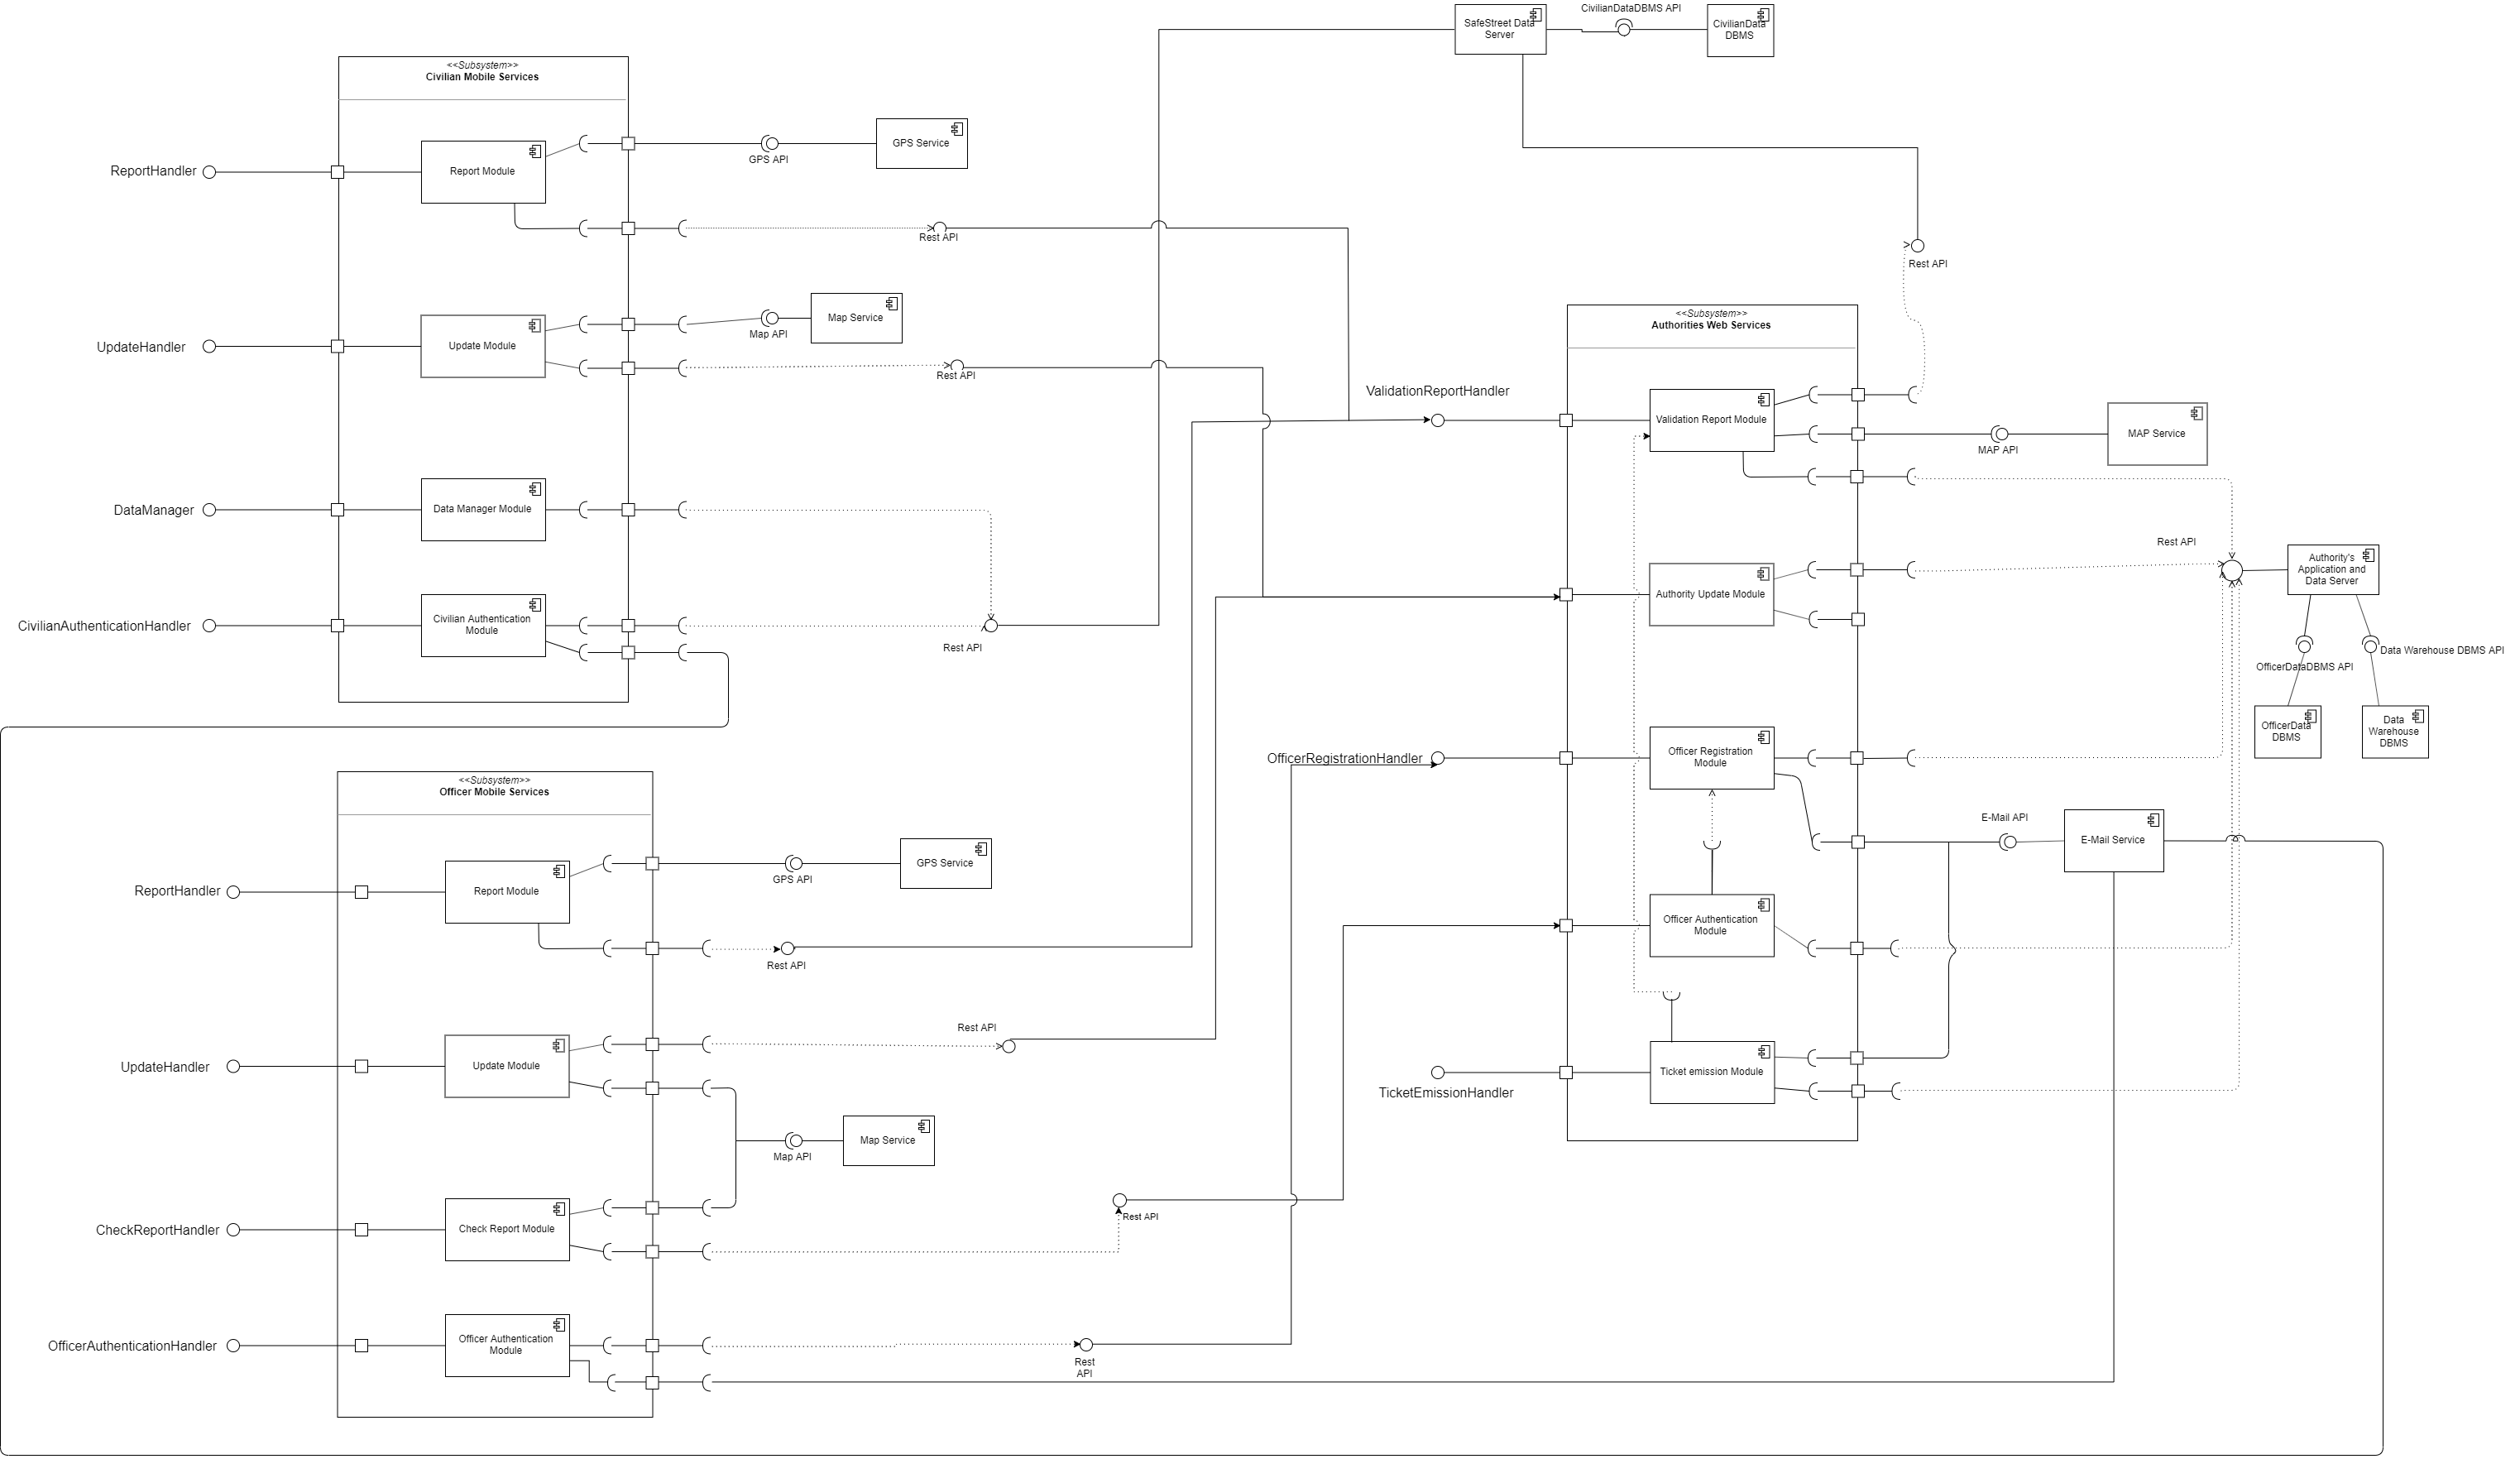
\includegraphics[width=0.95\paperwidth]{Images/OverallComponent}
					\end{adjustwidth}
			\end{figure}
\newpage
\subsection{Deployment view}
The architecture of the S2B, as shown in the component view paragraph, will be arranged in three tiers:
\begin{itemize}
\item \textbf{First tier:} is composed of the smartphones of the civilians and officers which run the mobile application, both in Android and iOS operative systems, and by the computer located at the Authority. All these clients communicate with the web server via HTTP thanks to a REST architecture, while mobile units can log in as civilians contacting the SafeStreets server.
\begin{figure}[H]
				\centering
					        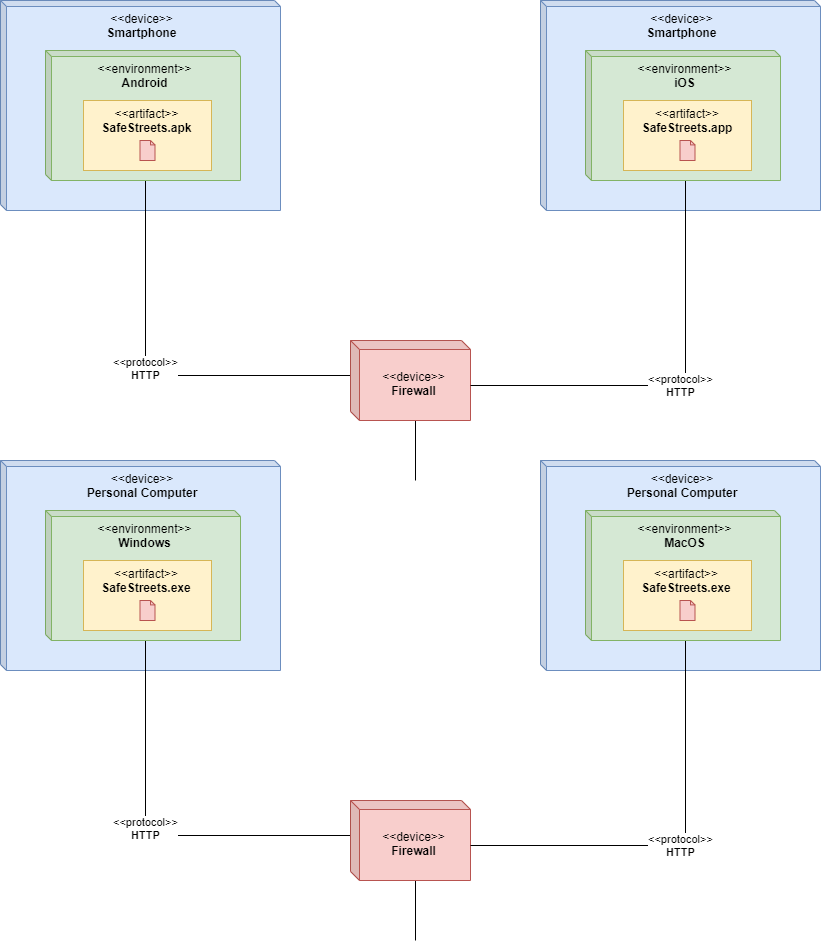
\includegraphics[width=0.6\paperwidth]{Images/firstTier}
			\end{figure}
\newpage
\item \textbf{Second tier:} is made of the Web Server which acts as a layer of communication for clients which want to interact with the ADS. We chose Apache Tomcat as web server as it is efficient and easy to implement through Spring Boot.
\begin{figure}[H]
				\centering				
					        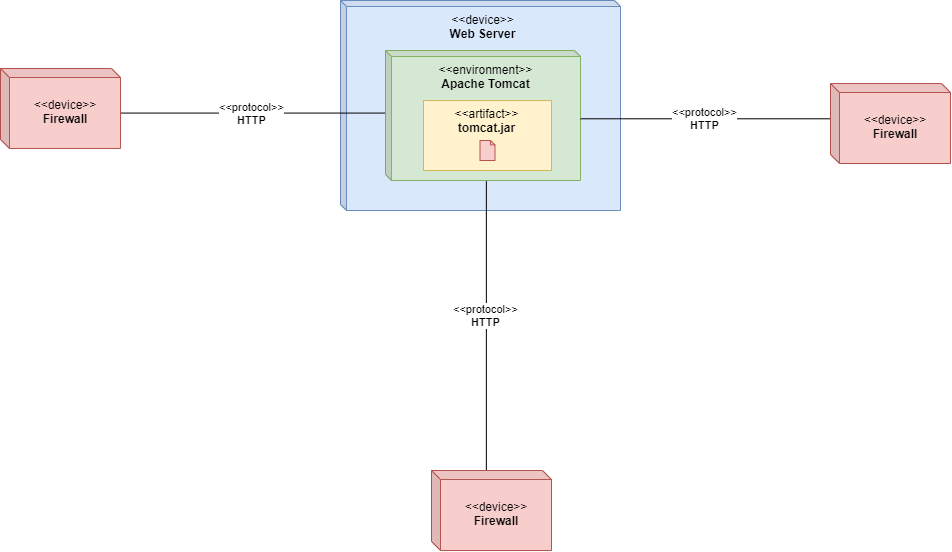
\includegraphics[width=0.7\paperwidth]{Images/secondTier}
			\end{figure}
\newpage
\item \textbf{Third tier:} the ADS with its application server and data servers, which communicate with the Officer Accounts database and with the Data Warehouse whose data is accessed through Hibernate which is again made easily interoperable with Spring Boot. The same implementation is used by the SafeStreet server which manages civilian accounts. We chose WildFly for the application servers because like Tomcat it provides a well documented and easily implementable framework.
\begin{figure}[H]
				\centering				
					        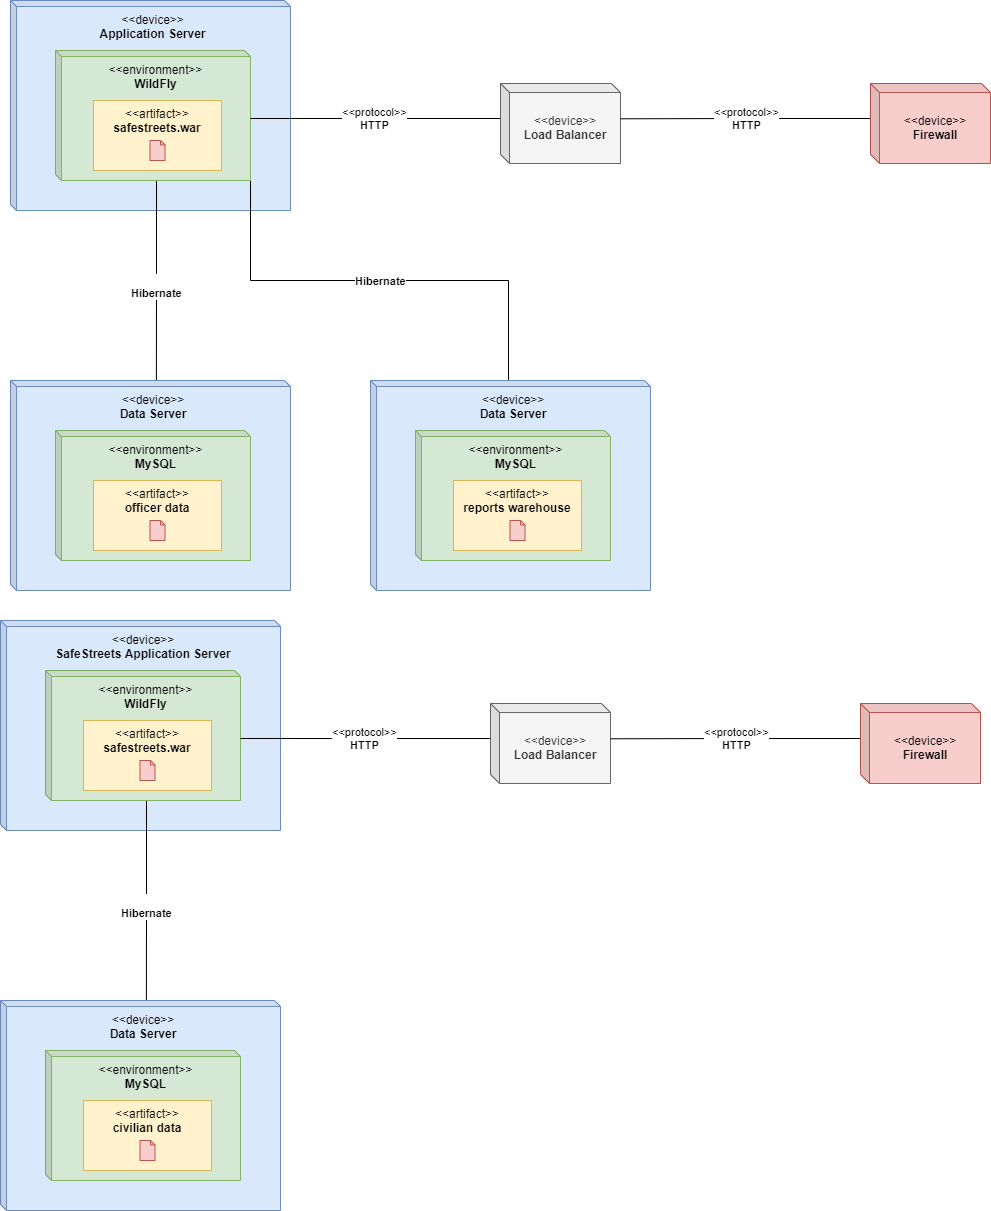
\includegraphics[width=0.6\paperwidth]{Images/thirdTier}
			\end{figure}
\end{itemize}
\newpage
This diagram represents the deployment view for the entire system:
\begin{figure}[H]
\begin{adjustwidth}{-25mm}{-25mm}
				\centering				
					        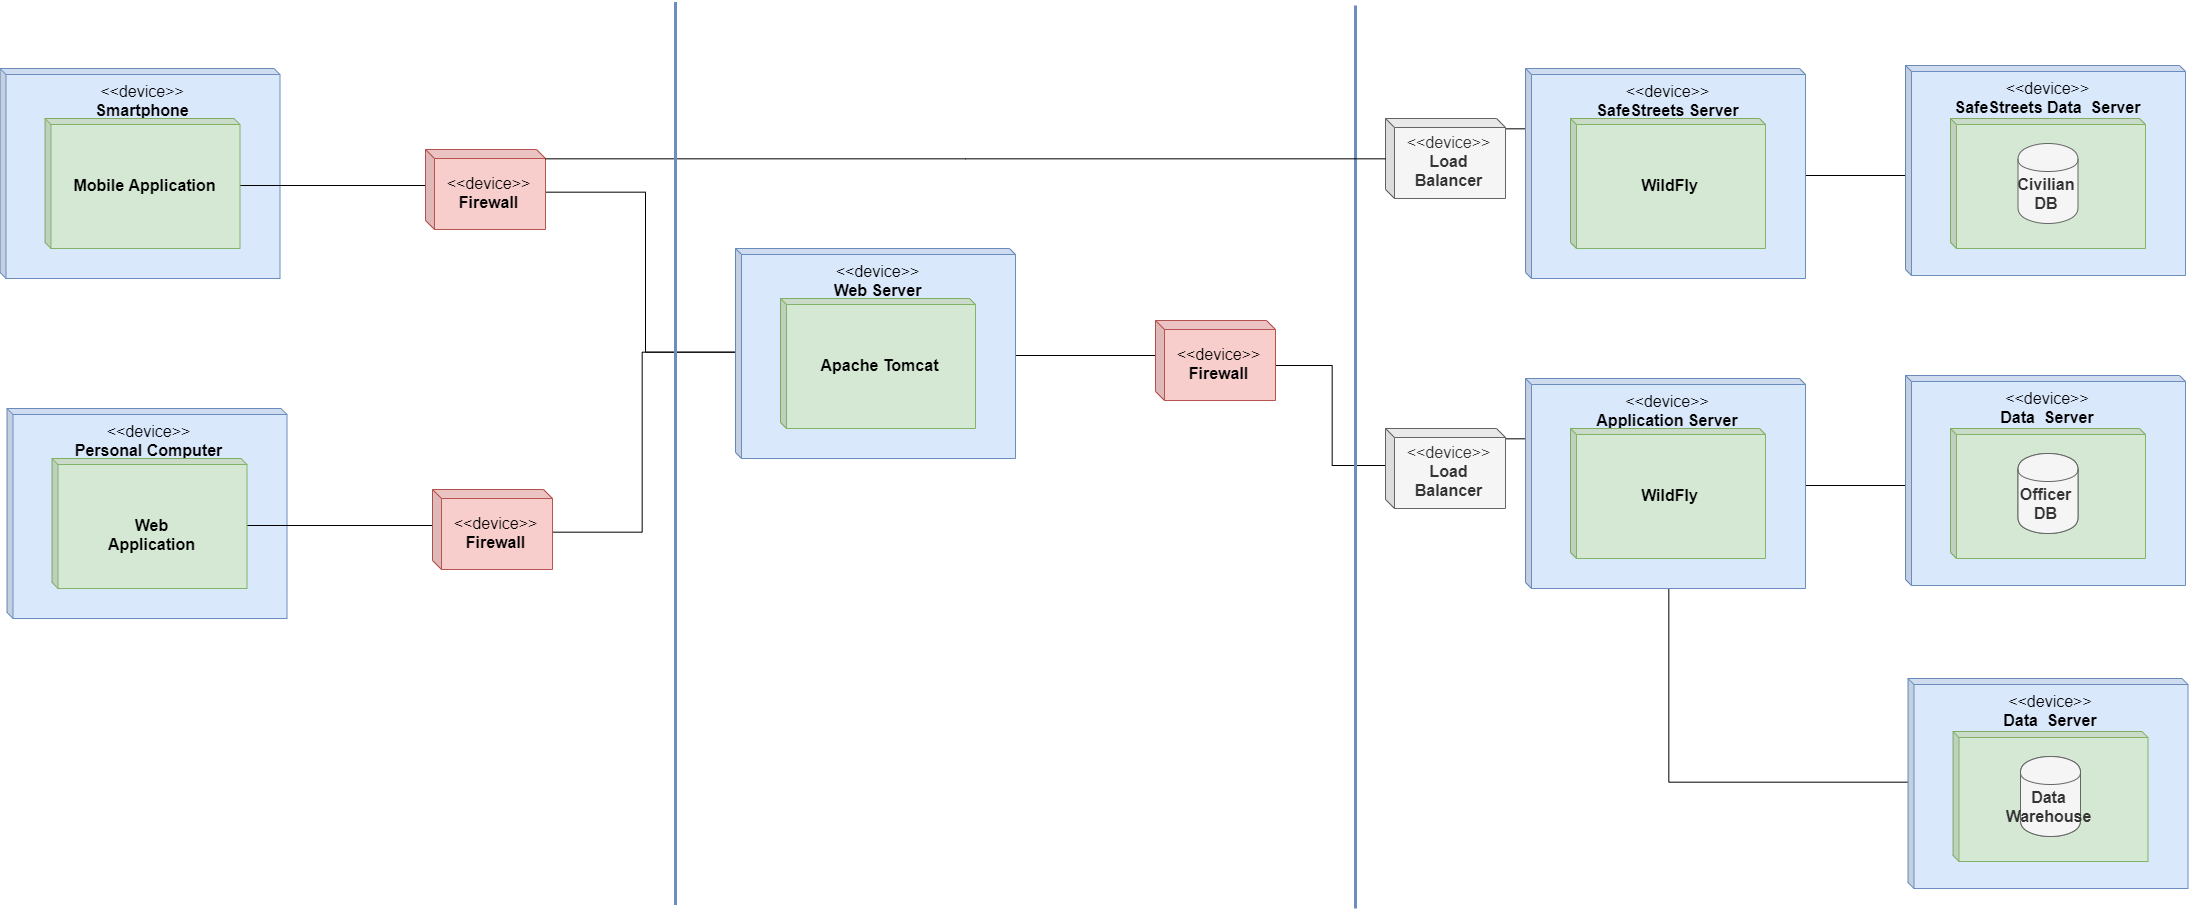
\includegraphics[width=0.9\paperwidth]{Images/deploymentView}
\end{adjustwidth}
			\end{figure}
\newpage
\subsection{Runtime view}
In this section we analyze the sequence diagram of the RASD expanded with further details regarding modules and components interacting.
\subsubsection{Civilian Registration}
\begin{figure}[H]
\begin{adjustwidth}{-25mm}{-25mm}
				\centering				
					        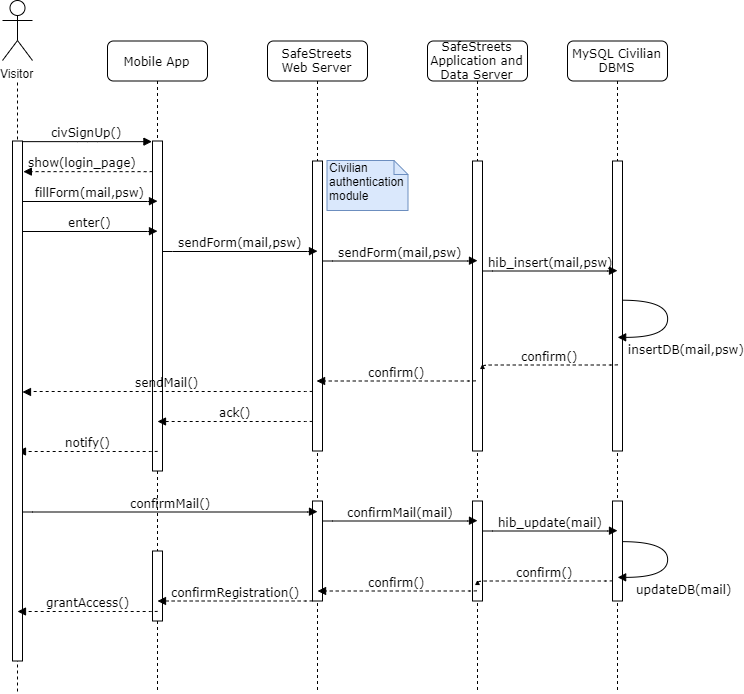
\includegraphics[width=0.5\paperwidth]{Images/Registration_sequence}
\end{adjustwidth}
\end{figure}
This sequence diagram describes the complete registration procedure of a civilian with no exceptions occurring, starting from the mobile app which sends the registration form through a HTTP Post message. This is received by the SafeStreets server thanks to their REST interface, and through the Hibernate API the software is able to interact with the MySQL DBMS which inserts the new tuple in the table for civilians account (after thorough encryption). We're able to determine if the operation has been correctly performed thanks to the result of the Hibernate method, and notify the mobile application of such outcome, and use the E-mail API to send a mail to the user. Once the registration has been confirmed, the server asks MySQL to update the tuple with some confirmation of the completed registration. All these processes are performed by the \texttt{Civilian Authentication Module} at the mobile app and SafeStreets server. The standard login procedure will be included in another diagram.
\subsubsection{Officer Registration}
\begin{figure}[H]
\begin{adjustwidth}{-25mm}{-25mm}
				\centering				
					        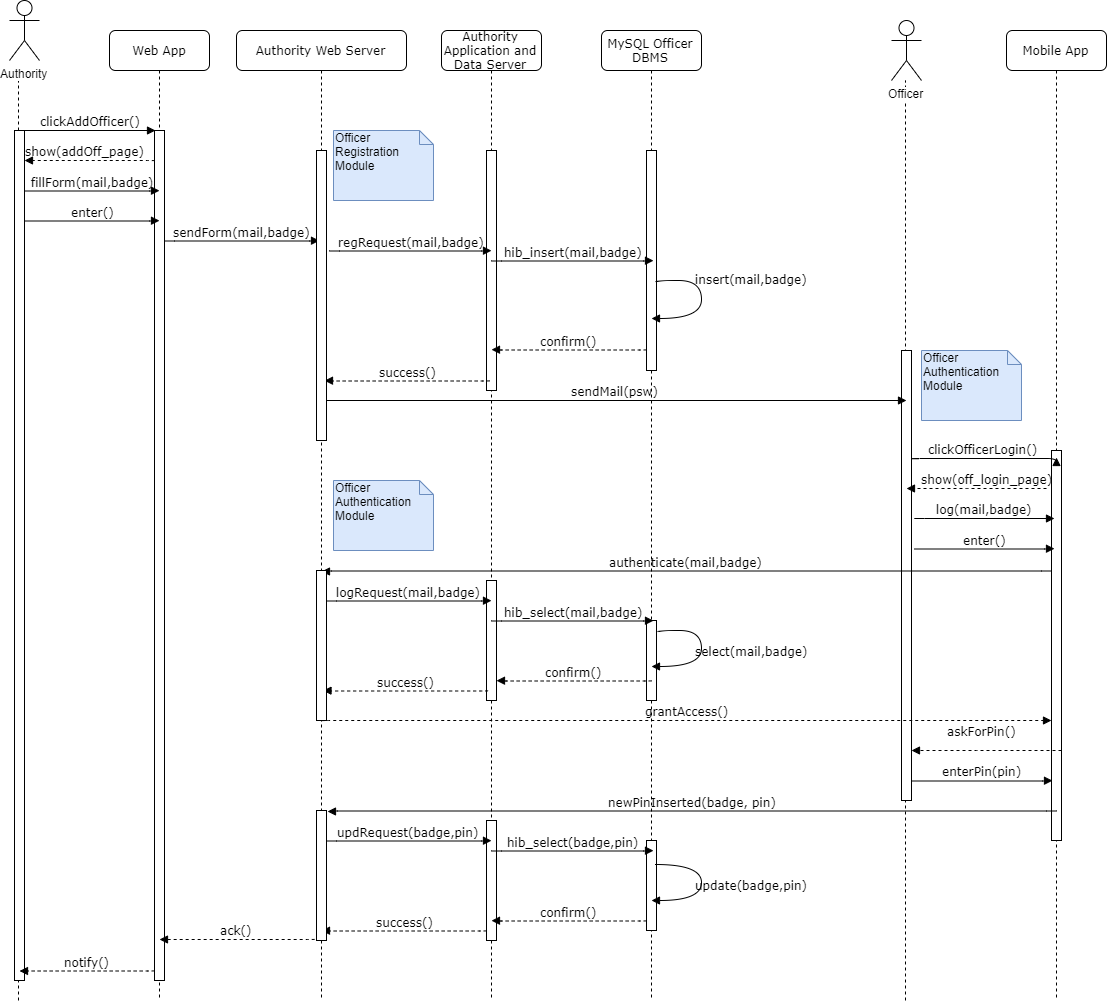
\includegraphics[width=0.75\paperwidth]{Images/Off_registration}
\end{adjustwidth}
\end{figure}
This one describes the full procedure of adding a new officer from the Authority's Web App. The request is forwarded through HTTP Post to the authority's web server which acts as the layer that has to be contacted to access to the ADS's functionalities. The ADS serves the request through the same kind of procedure explained in the previous sequence diagram. This first passage is handled by the \texttt{Officer Registration Module}. Once the officer has received the email with his password, he can successfully log in thanks to the \texttt{Officer Authentication Module}, and is after prompted to insert his secret pin to allow ticket emission. After the pin is inserted and iteratively forwarded to the ADS and stored, the officer can start using the application with full functionalities. The system forces the officer to insert the pin by checking (along with the log in request) if the pin has been already chosen or the officer still needs to insert it.
\subsubsection{Civilian Login and Report}
\begin{figure}[H]
\begin{adjustwidth}{-25mm}{-25mm}
				\centering				
					        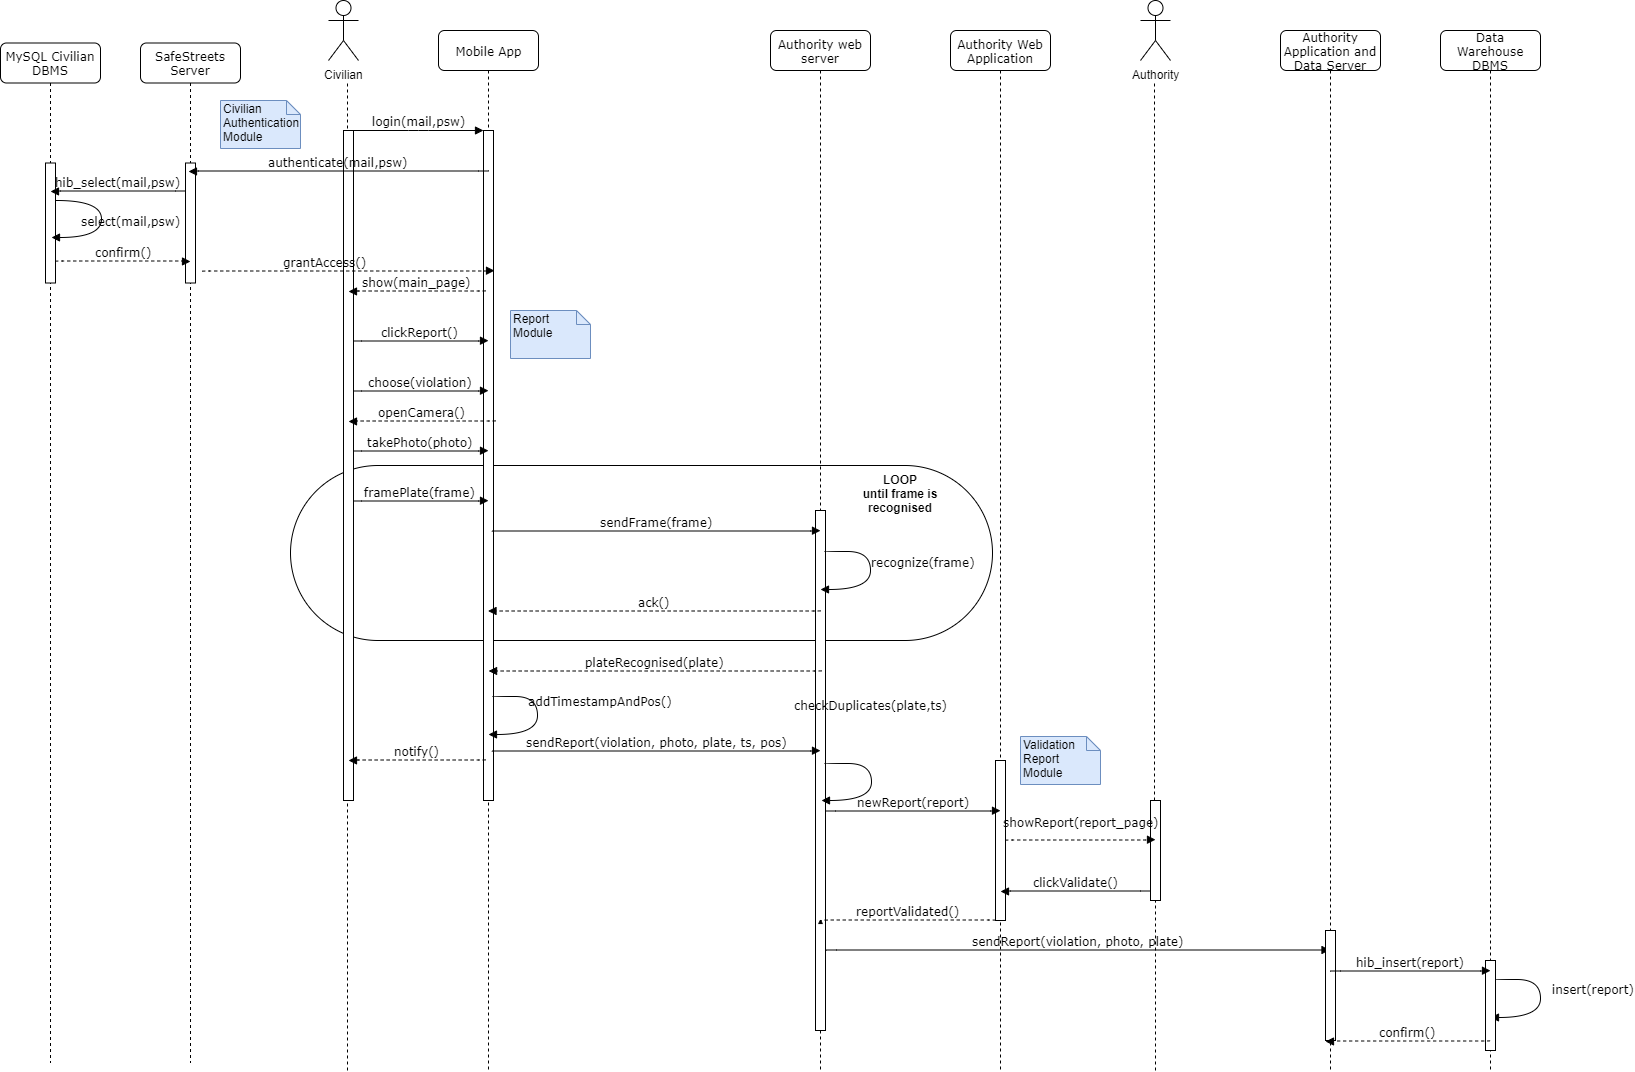
\includegraphics[width=0.75\paperwidth]{Images/Civilian_report}
\end{adjustwidth}
\end{figure}
The use case starts with the civilian successfully logging into the application through the standard procedure managed by the \texttt{Civilian Authentication Module}. The civilian decides to report a violation: chooses the type of violation and is subsequently prompted to take a photo of it. After that, he can start framing the plate with his camera: the various frames are sent to the Authority's Web server which analyses them until a plate number is recognized \textit{(this is the only application logic executed directly on the web server and not on the ADS for reduced latency)}. The Mobile Application then uses OS functionalities to stamp the report with time and coordinates, and the whole packet of data about the violation is sent to the web server through the REST interface. This entire process is handled by the \texttt{Report Modules} at the Mobile Application and at the Authority's web server. The personnel at the Authority's client can then validate it, triggering an exchange of messages with the ADS which culminates in the insertion of the report in the Data Warehouse. This final part is managed by the {Validation Report Module}. The newly added report will be subject to data mining and included in future updates sent by the ADS, but this will be included in another diagram.
\subsubsection{Report Invalidation and Banning}
\begin{figure}[H]
\begin{adjustwidth}{-25mm}{-25mm}
				\centering				
					        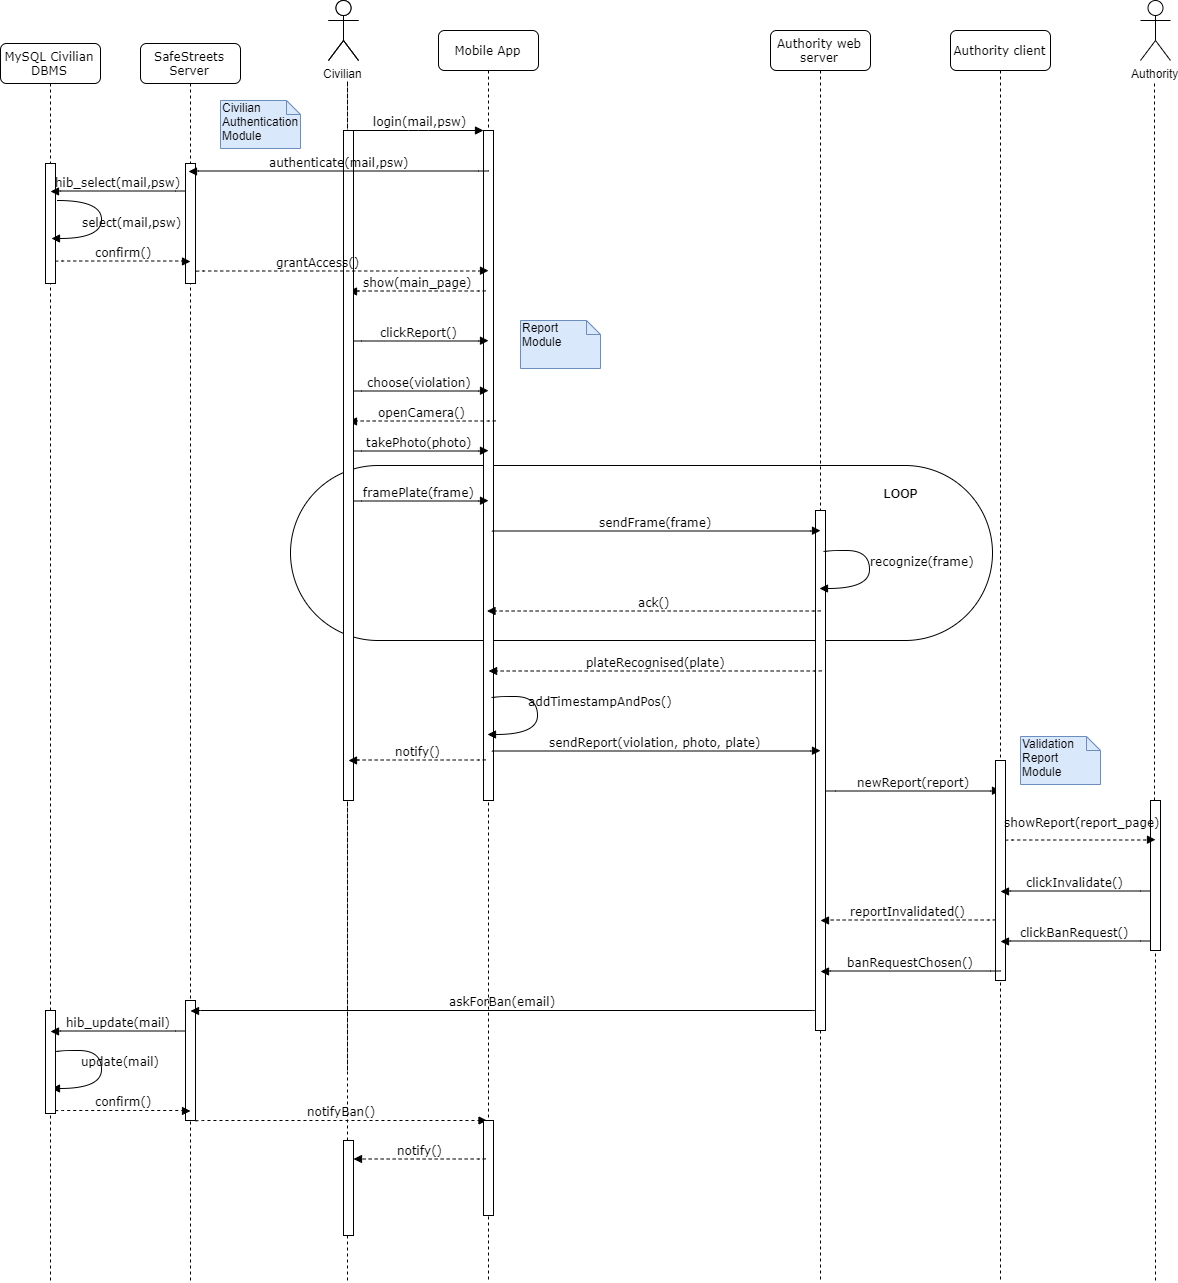
\includegraphics[width=0.75\paperwidth]{Images/invalidation_banning}
\end{adjustwidth}
\end{figure}
This use case includes all the same passages of the previous up to the report validation. In this case, the operator of the Authority's web application decides to invalidate the report which he deemed incorrect and request the ban of the user. The request is forwarded to the SafeStreets server which flags the user in his database thanks to the Hibernate API. The civilian is notified at the next access of the Mobile application of the ban, and the \texttt{Civilian Authentication Module} will take care of providing the effects of such measurement. It is important to notice the ADS isn't invoked in this sequence: that's because the ban is requested by the authority as a simple sending of messages, without any applicative logic at the authority's side, as the ban is served by the SafeStreets server which holds the civilian accounts database.
\subsubsection{Update spreading and Data Mining}
\begin{figure}[H]
\begin{adjustwidth}{-25mm}{-25mm}
				\centering				
					        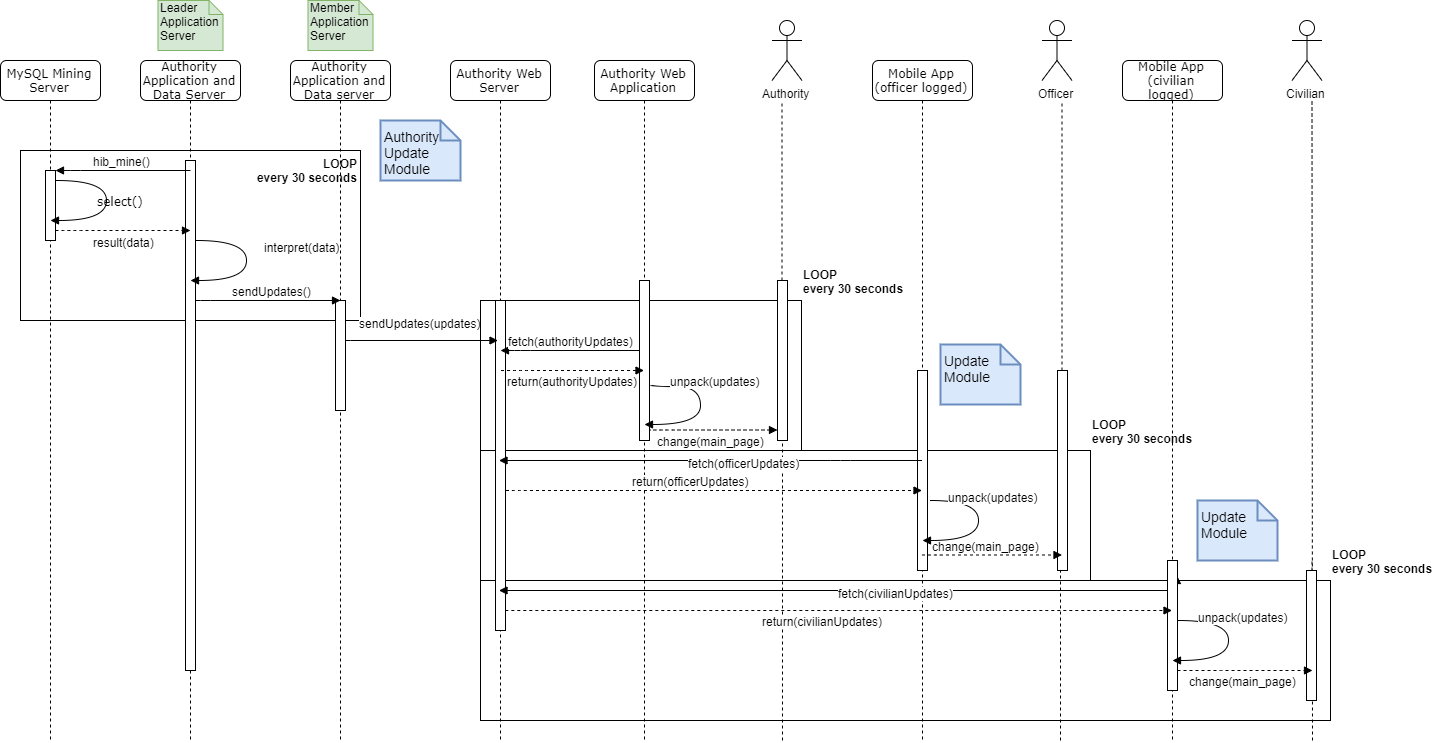
\includegraphics[width=0.75\paperwidth]{Images/update_sending}
\end{adjustwidth}
\end{figure}
This case covers the procedure of producing updates through data mining and spreading them in a network with ADSs distributed in a RAPS architecture. Through the \underline{bully election algorithm} a leader between the ADSs is chosen and is set as the root of a tree network with all the other ADSs as children: every 30 seconds he will query the database for relevant data, that he will pack into updates timestamped with a \underline{vector clock} and send to all the other connected ADSs. These will furtherly forward the messages to web servers in their domain. This is done by the \texttt{Authority Update Module}. Clients can fetch these updates from the Authority web server and retrieve the ones corresponding to them to preserve sensitive data, and unpack them to visualize the various information through their GUI. The mobile application does this with the \texttt{Update Module}.
\subsubsection{Ticket Emission}
\begin{figure}[H]
\begin{adjustwidth}{-25mm}{-25mm}
				\centering				
					        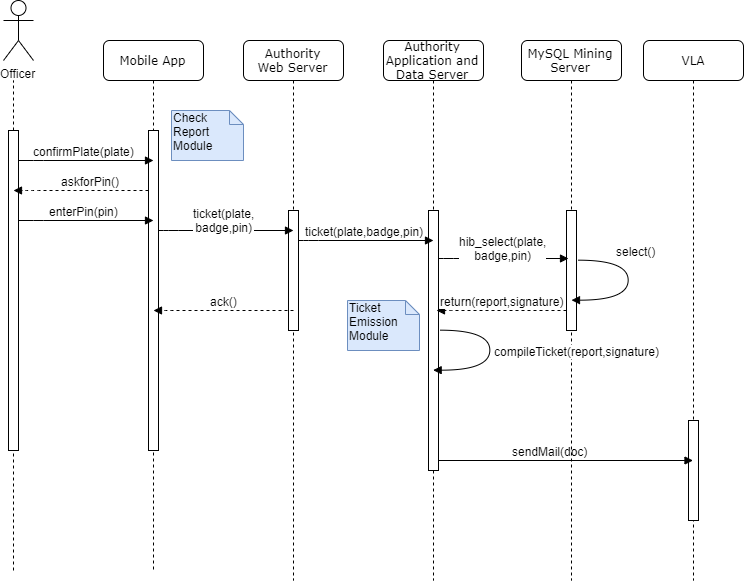
\includegraphics[width=0.75\paperwidth]{Images/automated_ticket}
\end{adjustwidth}
\end{figure}
This describes the interactions required to emit an automated ticket. As soon as the officer is near a report, he can confirm through the map the actual presence of a violation by verifying the correctness of the reported plate. As soon as he enters a secret pin a message is forwarded to the web server (all of this is performed by the \texttt{Check Report Module} then to the ADS which will query the report database to both authenticate the officer and find his signature, and the most recent report corresponding to the plate. If the query is successful, the ADS compiles a ticket and sends it via mail to the VLA. This involves the \texttt{Ticket Emission Module}.
\subsection{Component interfaces}
\subsubsection{External Interfaces}
SafeStreets will make use of some Application Programming Interfaces to simplify the implementation, since these components are largely used and compatible with the majority of the devices currently on the market:
\begin{itemize}
\item \texttt{Maps API} to have a visual representation of users' reports and HFVZs, to help Officers in finding a report that coud be confirmed or rejected. For our purpose the Google Maps API is perfectly suitable, since it can be embedded in both Android and iOS applications.
\item \texttt{GPS API} to geolocate the reports made by users and  avoid the possibility of forging the location, which could happen if users manually enters it. GPS will also provide the application with precise timestamps for the reports.
\item \texttt{REST API} as every distributed component will be provided with one, especially mobile clients will exploit it to interact with the web server at the Authority's location, which is the only layer visible to them. Also the SafeStreets data server's services and the ADS's will be invokable through a REST interface. Spring Boot, which uses Apache Tomcat as a web server, could be used as a versatile, easy to implement solution to build a functioning REST architecture across all subsystems.
\item \texttt{DBMS API} will be used to read and write all the database components:
\begin{itemize}
\item one at the SafeStreets server which manages civilian accounts;
\item one DW at the ADS location which holds records for all reports ever compiled and is queried to create the updates;
\item another one at the ADS location which manages officer accounts.
We will use MySQL as the DBMS, which will be manipulated directly from the software from the Hibernate API which can be easily configured to work with Spring Boot for simplicity and performance.
\end{itemize}
\item \texttt{E-Mail API} to send an Email to the officers added to the SafeStreets project and to send the compiled ticket to the VLA. 
\end{itemize}
\subsection{Architectural styles}
\subsubsection{RESTful architecture}
Our communication platform will be a client-server architecture based on the RESTful paradigm, which boasts great scalability and generality of interfaces, other than also being easy to implement and very self-descriptive. REST interfaces will be provided for every component to send and receive HTTP messages in a Object Oriented setting, where every communicating member exchanges and understands the same representations, which we decided to pack in a \texttt{JSON} format. We will make messages as self-descriptive as possible to describe the service being called or the messages being exchanged. Morevorer, there are several frameworks which contain their own REST-related libraries such as Spring Boot, which significantly reduces implementation time and complexity.
\subsubsection{RACS and RAPS}
The functionalities of the SafeStreets server will be cloned across different machine to provide better load balancing, fault tolerance, reliability and availability. Thus the servers will be arranged in a \texttt{RACS} architecture. For what concerns the ADSs, in settings like bigger cities with a greater user base, the services could be partitioned in microservices across different machines (therefore in a \texttt{RAPS} architecture), for instance by making a machine serve ticket emissions, another one officer account functionalities, and another one to serve updates, or each machine could serve a bounded amount of Authorities' web servers (in this case it should better be defined as a \texttt{RACS} architecture as the services across all the machines are the same, they're simply designed to serve a different requestor).
\subsection{Patterns and design decisions}
\subsubsection{MVC}
We decided to utilize \texttt{Model-View-Controller} as the pattern to model the software architecture, as it allows for simplified implementation, mainteinability and security. For example, from the perspective of the authority, we could see the view package as the GUI, the controller as the REST interface which calls and receives all the calls which will eventually result in functions being run in the model held in the ADS. An analogous argument could be made from the perspective of users. 
\subsubsection{Bully Election algorithm}
As having multiple ADSs mine the same data and produce the same reports is, computationally speaking, a waste of resources, we decided the ADSs will be arranged in a rooted tree network with synchronous communication and a leader ADS as root. This leader will be elected through the \texttt{Bully election algorithm} which is generally considered an efficient enogh solution and doesn't use too much overhead to accomplish the task. IDs to servers will be assigned in ascending order based on the performance of the physical machine, so that the algorithm tries to elect the most performing server.
\subsubsection{Distributed Transactions and Mutual Exclusion}
It will be important to ensure concurrent accesses to the databases do not violate integrity constraints. Mutual exclusion and distributed commit protocols are known to be as important as they are difficult to implement, thus we decided to utilize \texttt{Hibernate} (which is based on \texttt{JDBC}) as our framework to manage read and write accesses, as it is known to guarantee mutual exclusion and sufficient parallelism in distributed transaction. This way no time and effort will be used by the developers to code these functionalities directly from Java primitives.
\subsubsection{Update propagation strategy}
The leader, after mining the updates, will stamp each one of them with a vector clock to perform \underline{causally ordered multicast} (so that no updates are temporally misplaced by the final users), and follow a \texttt{push based anti-entropy propagation strategy} to spread the updates to all the ADSs in his network, that will do the same by forwarding them to their connected web servers. At this point, every time a client needs an update, it may be after a timer going off or some condition being satisfied, it can simply fetch the update from its connected web server (this time it's \texttt{pull based} to avoid wasting of resources). The web server knows what kind of actor is trying to retrieve the updates and will only give out the permitted ones. 
\newpage
\section{USER INTERFACE DESIGN}
As various mockups of the design of the clients were already included in chapter 3 of the \texttt{Requirement Analysis and Specification Document}, we decided to include the User Experience diagrams which describe the ways with which the various actors interact with their GUIs. For further details on how the clients will work, it is possible to refer to the Statecharts in chapter 2 of the RASD.
\\
\subsection{Civilian UX}
When civilians launch the app on their mobile phone the first page they visualize is the Start Menu. Here they can authenticate themselves (both login and registration).
Regarding the registration they must insert their data and confirm the email received, while for login they have to insert their authentication data. Once they are logged in they can visualize the map, the statistics or modify their login data. In the map menu they can compile a report with the previously described procedure, while in the statistics menu they can visualize the data received through the updates, about their report, HFVZs and data about all the reports.
\begin{figure}[H]
		\centering
			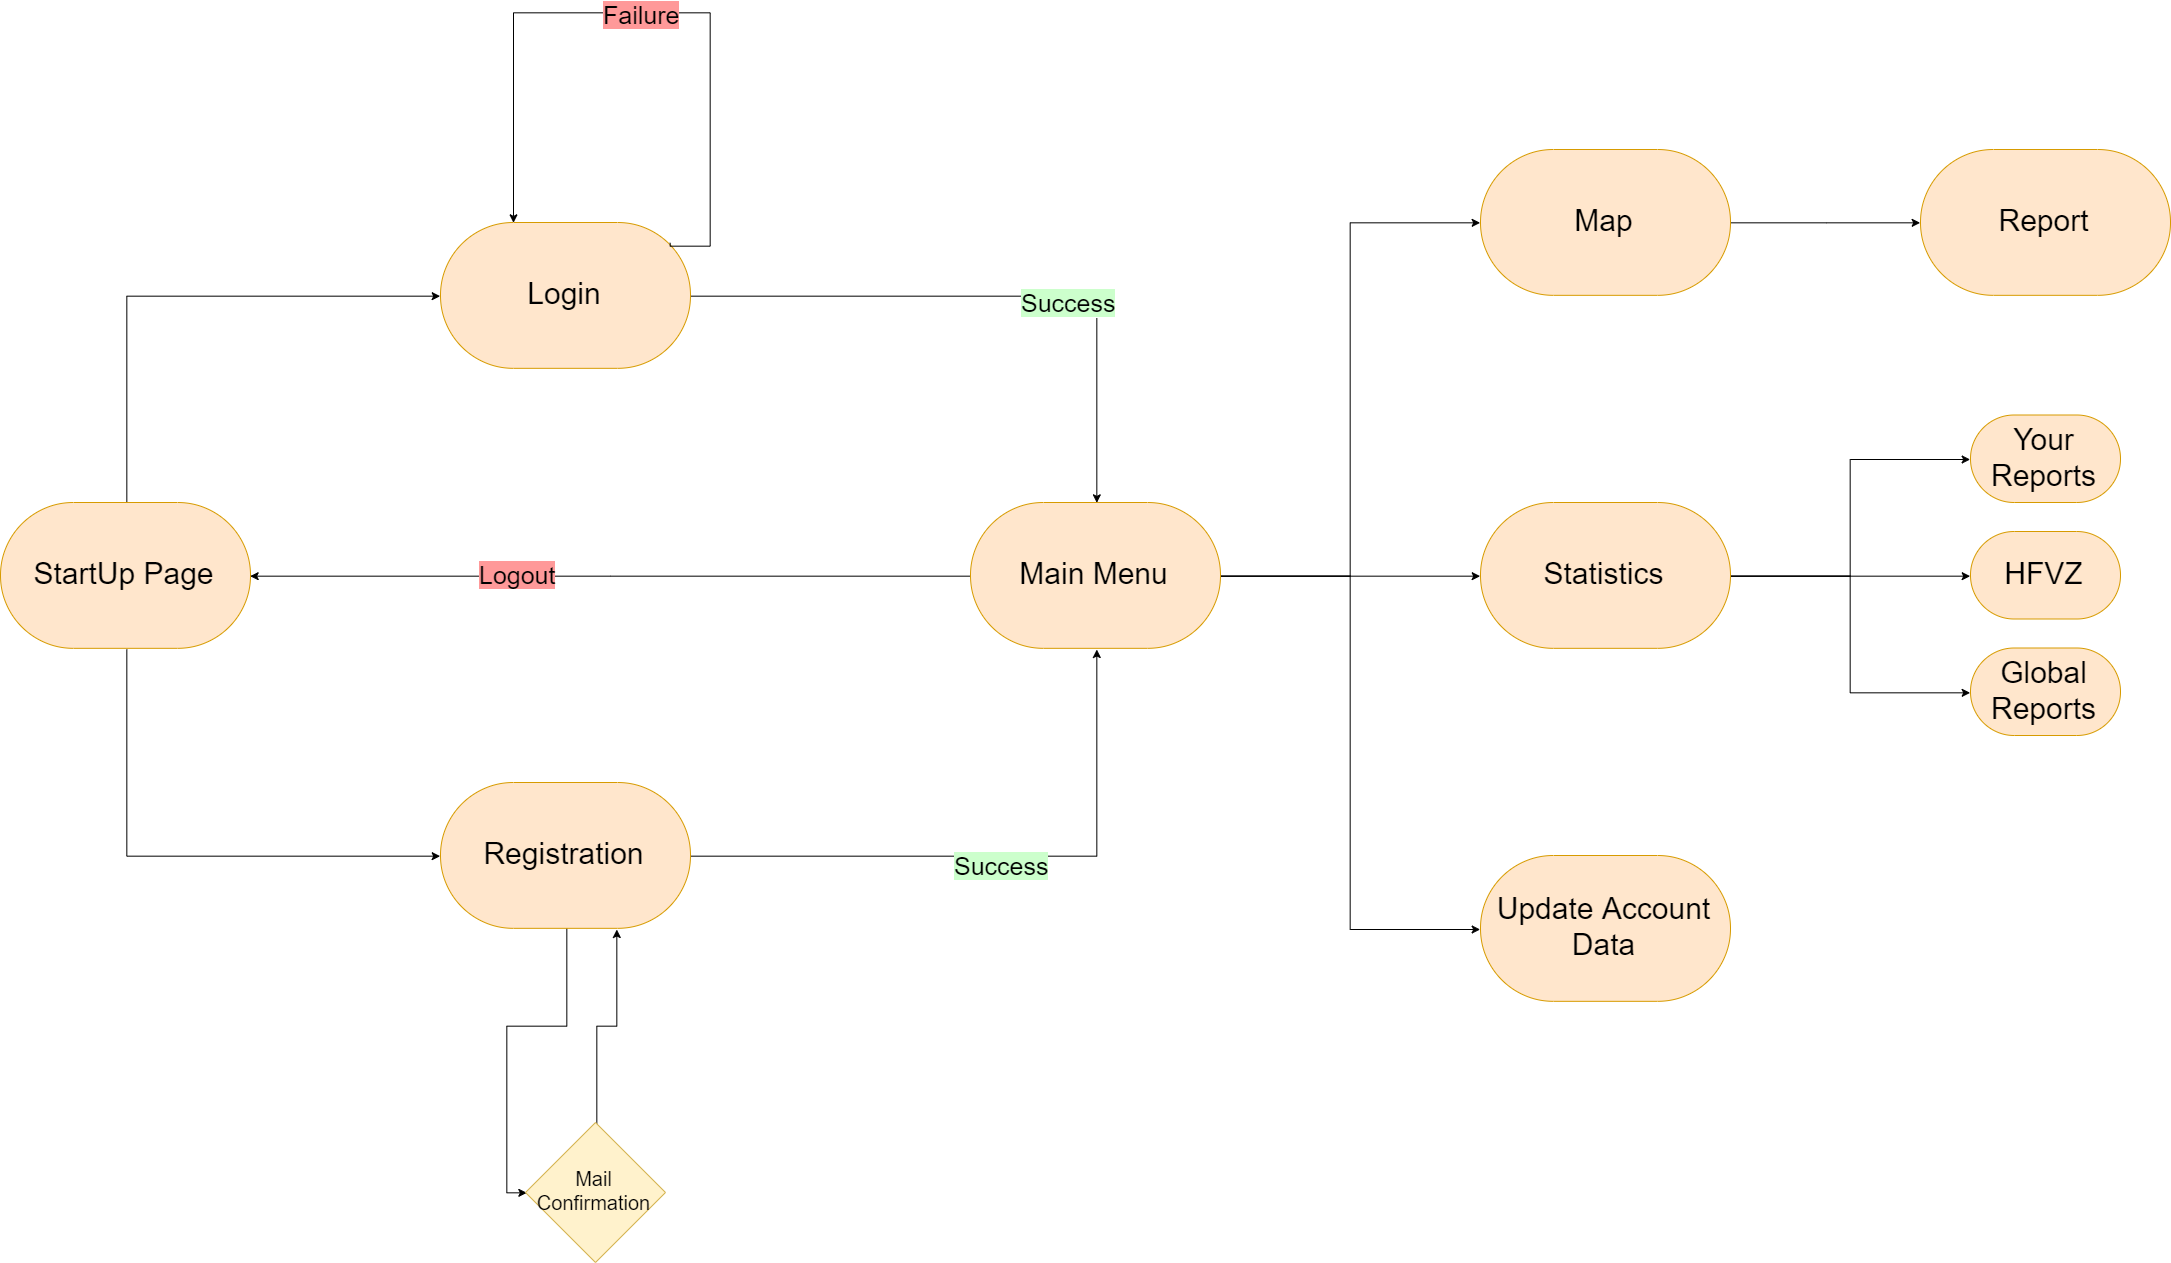
\includegraphics[width=1.2\linewidth]{Images/UX/CivilianUX}
\end{figure}
\newpage
\subsection{Officer UX}
The mobile application seen by officers is pretty much the same as the one seen by civilians. Officers can login by using their badge ID and the password communicated by email (this is triggered by the Authority which added the officer). For the first login, the officer is required to choose a PIN so he will be able to eventually confirm reports for ticket emission. After this, he can visualize the Map and the statistics. The statistics are the same of the civilians, plus the Repeat Offenders. On the map he can compile or check a report throught the relative buttons; moreover, if he checks a report and the violation occured he can allow the sending of a traffic ticket to the VLA by compiling the form which requires the insertion of his PIN. If the violation doesn't match the report data, or is no longer present, the officer can reject the report and prompt the ADS to remove it from the map.
\begin{figure}[H]
		\centering
\begin{adjustwidth}{-25mm}{-25mm}
					        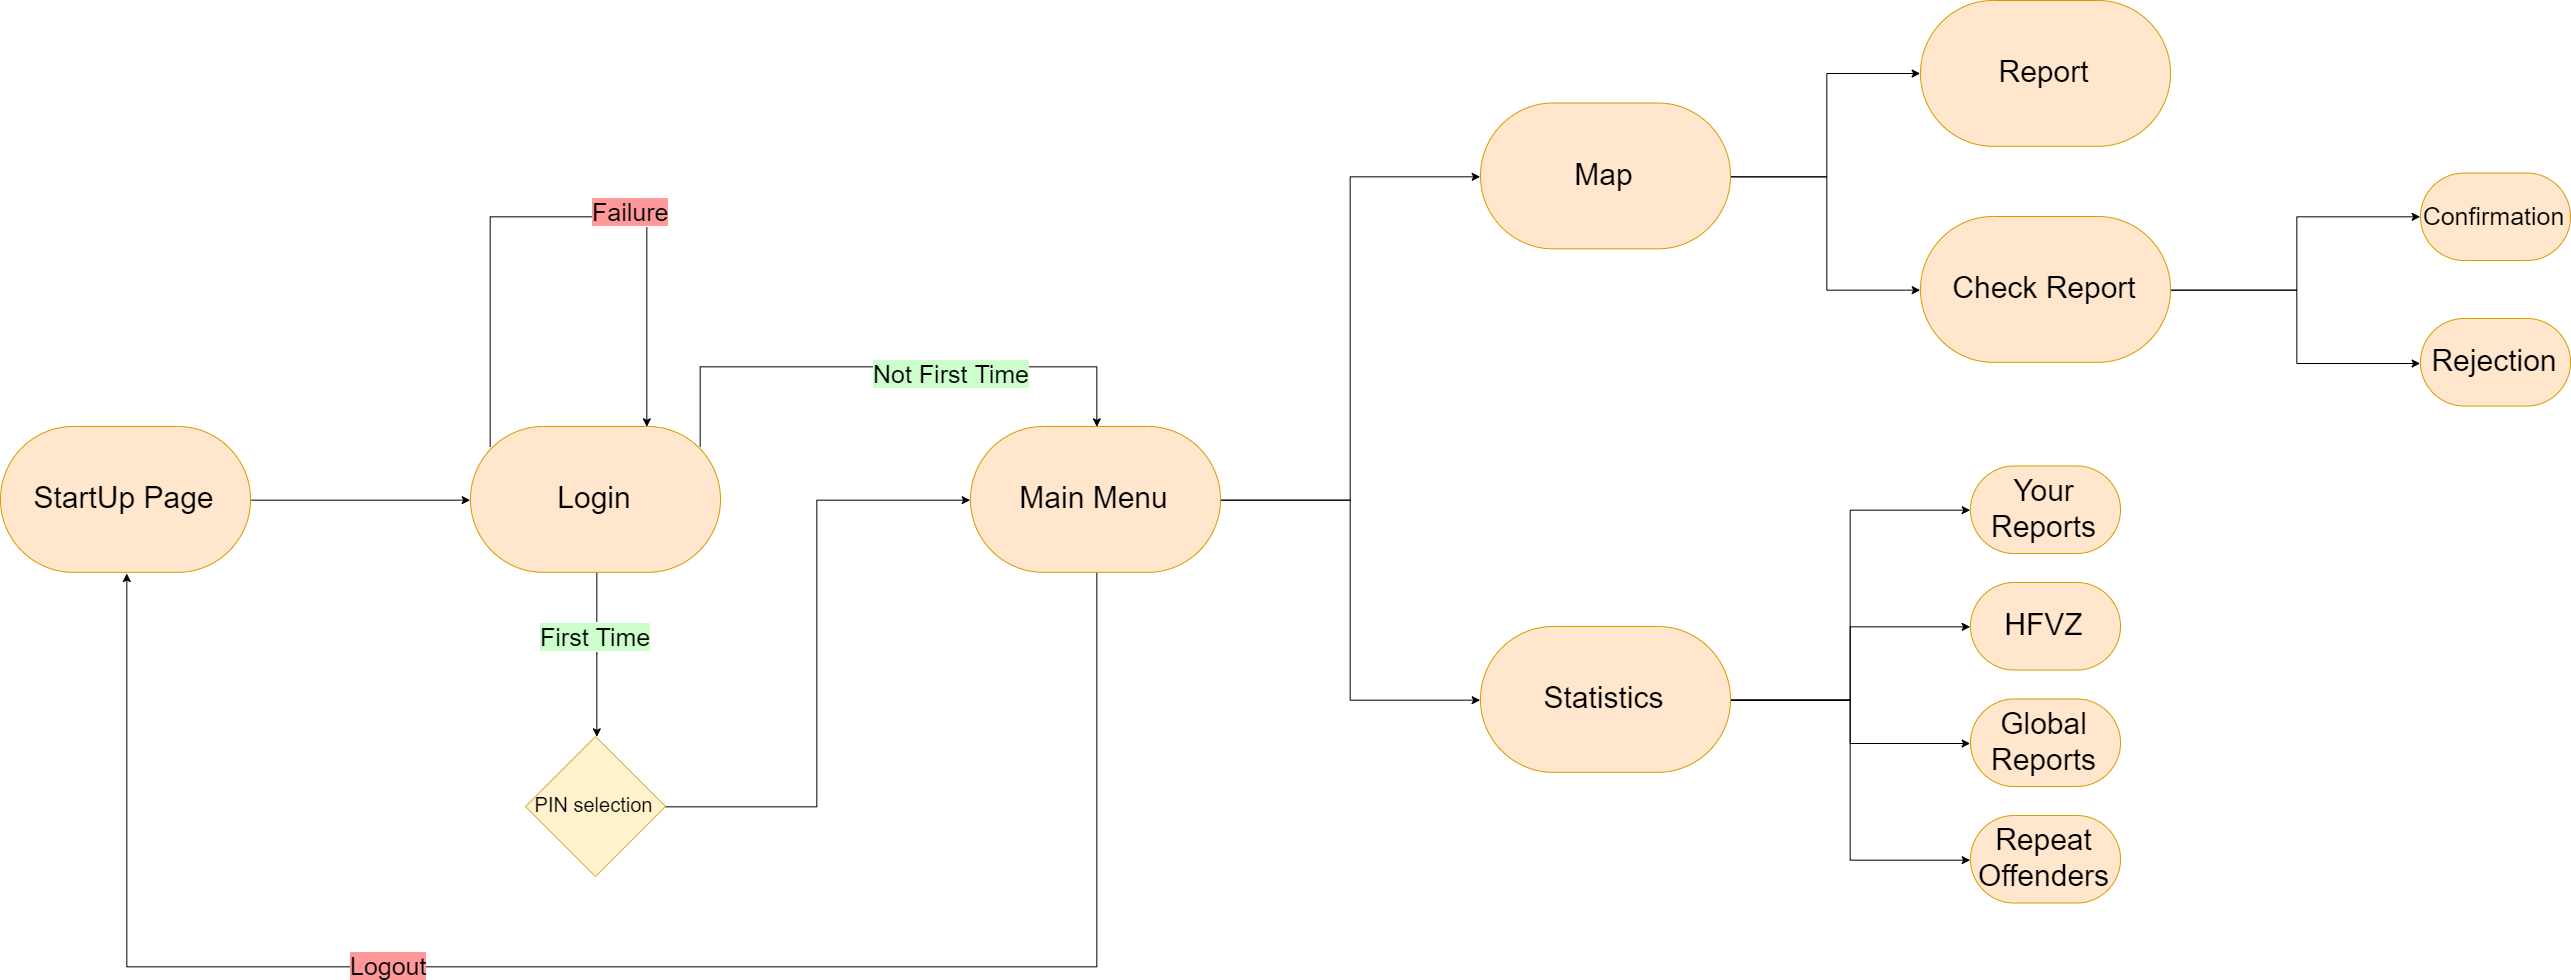
\includegraphics[width=1\linewidth]{Images/UX/OfficerUX}
					\end{adjustwidth}		
	
\end{figure}
\newpage
\subsection{Authority UX}
The authorities work on a web application. From this application they can add officers to the SafeStreets system by sending them an email with the purpose of program and an automatically generated password to allow officers to login along with their badge ID. The authoritiescan  also check the data sent by users' reports and confirm or reject them. They can also send a ban request for a civilian to the SafeStreets staff. They can also visualize the same statistics of the officers.
\begin{figure}[H]
		\centering
			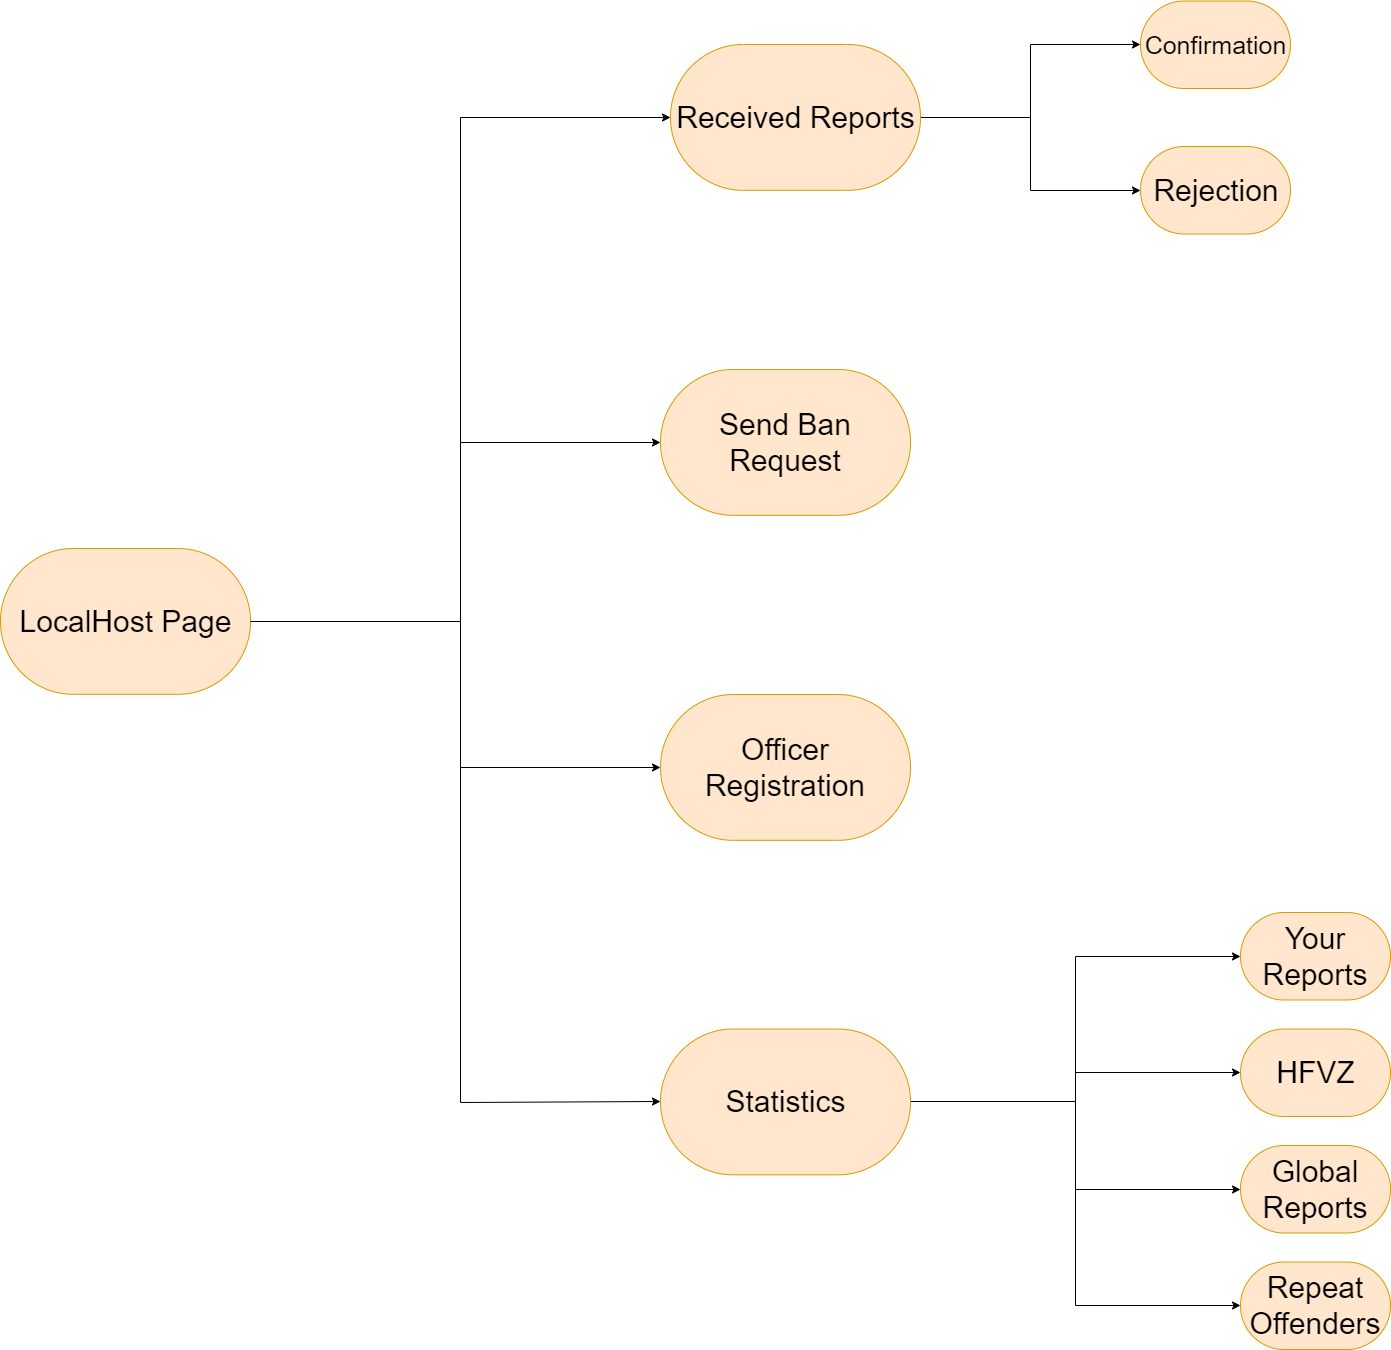
\includegraphics[width=0.75\linewidth]{Images/UX/AuthorityUX}
\end{figure}
\newpage
\section{REQUIREMENTS TRACEABILITY}
In this section is highlighted the link between the requirements stated in the RASD and the components listed in the section 2.2.\\\\

\textbf{[R1]: Separate civilian and officer registration and login functionality.}
\begin{itemize}
	\item \texttt{Referring Goal}
	\begin{itemize}
		\item G1
		\item G5.2
	\end{itemize}
	\item \texttt{Component}
	\begin{itemize}
		\item Officer Registration Module 	\item Officer Authentication Module 	\item Civilian Authentication Module
	\end{itemize}
\end{itemize}
\textbf{	[R2]: Data has to be correctly queried server-side everytime, to make sure no duplicate accounts are created or no unregistered visitors log in. }
\begin{itemize}
	\item \texttt{Referring Goal}
	\begin{itemize}
		\item G1
	\end{itemize}
	\item \texttt{Component}
	\begin{itemize}
		\item Officer Registration Module
		\item Officer Authentication Module
		\item Civilian Authentication Module
	\end{itemize}
\end{itemize}
\textbf{[R3]: Send confirmation emails within at most one minute after the registration confirmation receipt (or the new officer being added). }
\begin{itemize}
	\item \texttt{Referring Goal}
	\begin{itemize}
		\item G1
	\end{itemize}
	\item \texttt{Component}
	\begin{itemize}
		\item Officer Registration Module 	\item Civilian Authentication Module
	\end{itemize}
\end{itemize}
\textbf{[R4]: Confirm user registration within at most one minute after the email link has been clicked.}
\begin{itemize}
	\item \texttt{Referring Goal}
	\begin{itemize}
		\item G1
	\end{itemize}
	\item \texttt{Component}
	\begin{itemize}
		\item Officer Registration Module
		\item Civilian Authentication Module
	\end{itemize}
\end{itemize}
\textbf{[R5]: Force the user to allow the S2B to access the device's camera and GPS.}
\begin{itemize}
	\item \texttt{Referring Goal}
	\begin{itemize}
		\item G2
	\end{itemize}
	\item \texttt{Component}
	\begin{itemize}
		\item Report Module
		\item Update Module
	\end{itemize}
\end{itemize}
\textbf{[R6]: Implement a function in the authority's client which allows personnel to validate or invalidate reports.}
\begin{itemize}
	\item \texttt{Referring Goal}
	\begin{itemize}
		\item G2
		\item G5.1
	\end{itemize}
	\item \texttt{Component}
	\begin{itemize}
		\item Validation Report Module
	\end{itemize}
\end{itemize}
\textbf{[R7]: Implement a supervised learning algorithm server-side which scans the multiple frames sent by the user to recognize the license plate.}
\begin{itemize}
	\item \texttt{Referring Goal}
	\begin{itemize}
		\item G2
		\item G5.1
	\end{itemize}
	\item \texttt{Component}
	\begin{itemize}
	\item Report Module
		\item Validation Report Module
	\end{itemize}
\end{itemize}
\textbf{[R8]: Automatically discard the report if another one with the same plate has been received within an hour to avoid duplicates.}
\begin{itemize}
	\item \texttt{Referring Goal}
	\begin{itemize}
		\item G2
		\item G5.1
	\end{itemize}
	\item \texttt{Component}
	\begin{itemize}
			\item Validation Report Module
	\end{itemize}
\end{itemize}
\textbf{[R9]: The supervised learning algorithm must be accurate at least 99\% of the times.}
\begin{itemize}
	\item \texttt{Referring Goal}
	\begin{itemize}
		\item G2
		\item G5.1
	\end{itemize}
	\item \texttt{Component}
	\begin{itemize}	
	\item Validation Report Module		\end{itemize}
\end{itemize}
\textbf{[R10]: Acknowledgments from the authority's server must be received within 10 seconds.}
\begin{itemize}
	\item \texttt{Referring Goal}
	\begin{itemize}
		\item G2
	\end{itemize}
	\item \texttt{Component}
	\begin{itemize}
		\item Validation Report Module
	\end{itemize}
\end{itemize}
\textbf{[R11]: Store the report info in the DW everytime it is confirmed to be valid.}
\begin{itemize}
	\item \texttt{Referring Goal}
	\begin{itemize}
		\item G3
	\end{itemize}
	\item \texttt{Component}
	\begin{itemize}
		\item Authority Update Module
	\end{itemize}
\end{itemize}
\textbf{[R12]: Make the data warehousing and processing completely invisible to human actors to avoid manipulations.}
\begin{itemize}
	\item \texttt{Referring Goal}
	\begin{itemize}
		\item G3
	\end{itemize}
	\item \texttt{Component}
	\begin{itemize}
		\item Authority Update Module
	\end{itemize}
\end{itemize}
\textbf{[R13]: implement functionality which allows (through the authority's client) to toggle automatic tickets ON or OFF.}
\begin{itemize}
	\item \texttt{Referring Goal}
	\begin{itemize}
		\item G4.1
	\end{itemize}
	\item \texttt{Component}
	\begin{itemize}
		\item Ticket Emission Module
	\end{itemize}
\end{itemize}
\textbf{[R14]: force newly logged officers to choose a 5 digit pin to release tickets.}
\begin{itemize}
	\item \texttt{Referring Goal}
	\begin{itemize}
		\item G4.1
	\end{itemize}
	\item \texttt{Component}
	\begin{itemize}
		\item Officer Registration Module
	\end{itemize}
\end{itemize}
\textbf{[R15]: implement functionality which allows officers' near a report to confirm both the report itself and the ticket emission through the pin.}
\begin{itemize}
	\item \texttt{Referring Goal}
	\begin{itemize}
		\item G4.1
	\end{itemize}
	\item \texttt{Component}
	\begin{itemize}
		\item Check Report Module
		\item Ticket Emission Module
	\end{itemize}
\end{itemize}
\textbf{[R16]: implement functionality which uses report data and the officer's signature to compile a ticket and send it to the VLA via email.}
\begin{itemize}
	\item \texttt{Referring Goal}
	\begin{itemize}
		\item G4.1
	\end{itemize}
	\item \texttt{Component}
	\begin{itemize}
		\item Check Report Module
		\item Ticket Emission Module
	\end{itemize}
\end{itemize}
\textbf{[R17]: update every actor's map with the HFVZs every 30 seconds.}
\begin{itemize}
	\item \texttt{Referring Goal}
	\begin{itemize}
		\item G4.2
	\end{itemize}
	\item \texttt{Component}
	\begin{itemize}
		\item Update Module
		\item Authority Update Module 
	\end{itemize}
\end{itemize}
\textbf{[R18]: update only the authorities' and officers' maps with the new reports and repeat offenders lists in real time.}
\begin{itemize}
	\item \texttt{Referring Goal}
	\begin{itemize}
		\item G4.2
		\item G6
	\end{itemize}
	\item \texttt{Component}
	\begin{itemize}
		\item Authority Update Module 
	\end{itemize}
\end{itemize}
\textbf{[R19]: show repetead offenders in real time in the authorities' GUI.}
\begin{itemize}
	\item \texttt{Referring Goal}
	\begin{itemize}
		\item G4.2
	\end{itemize}
	\item \texttt{Component}
	\begin{itemize}
		\item Authority Update Module 
	\end{itemize}
\end{itemize}
\textbf{[R20]: Make sure officers can only be added through the Authority's client.}
\begin{itemize}
	\item \texttt{Referring Goal}
	\begin{itemize}
		\item G5.2
	\end{itemize}
	\item \texttt{Component}
	\begin{itemize}
		\item Officer Registration Module
	\end{itemize}
\end{itemize}
\textbf{[R21]: Officers can only log into the app through a combination of Badge ID and a password received via email by the Authority.}
\begin{itemize}
	\item \texttt{Referring Goal}
	\begin{itemize}
		\item G5.2
		\item G5.3
	\end{itemize}
	\item \texttt{Component}
	\begin{itemize}
		\item Officer Registration Module
		\item Officer Authentication Module
	\end{itemize}
\end{itemize}
\textbf{[R22]: Officers can only allow automated ticket emission by entering their secret pin.}
\begin{itemize}
	\item \texttt{Referring Goal}
	\begin{itemize}
		\item G5.3
	\end{itemize}
	\item \texttt{Component}
	\begin{itemize}
		\item Check Report Module
		\item Ticket Emission Module	
	\end{itemize}
\end{itemize}
\textbf{[R23]: Officers are automatically required to login every 6 hours and their access data can't be autofilled.}
\begin{itemize}
	\item \texttt{Referring Goal}
	\begin{itemize}
		\item G5.3	
	\end{itemize}
	\item \texttt{Component}
	\begin{itemize}
		\item Officer Authentication Module 
	\end{itemize}
\end{itemize}
\textbf{[R24]: A ban request can be issued through the Authority's client after receiving an invalid report.}
\begin{itemize}
	\item \texttt{Referring Goal}
	\begin{itemize}
		\item G5.4
	\end{itemize}
	\item \texttt{Component}
	\begin{itemize}
		\item Validation Report Module 
	\end{itemize}
\end{itemize}
\textbf{[R25]: The S2B must comply with GDPR rules.}
\begin{itemize}
	\item \texttt{Referring Goal}
	\begin{itemize}
		\item G6
	\end{itemize}
	\item \texttt{Component}
	\begin{itemize}
		\item Data Manager Module 
	\end{itemize}
\end{itemize}
\section{Implementation, Integration and Test Plan}
		\subsection{Implementation Plan}
		The implementation of our system will be done following a bottom-up approach that will facilitate a high deployment coverage in early phases. The order in which our implementation will be carried out, takes in account different factors such as the complexity of the modules and how they are interconnected with one another and we must take in consideration the possibility of discovering flaws and bugs in our designed system that will require to be fixed as soon as possible in order to prevent further additional costs and difficulties in debugging.\\ It will also be vital to distinguish basic application features which will appear in the MVP of the application, as we'd rather follow the lean approach to development instead of a waterfall solution. All the hardware components (specified in the deployment view) are assumed to be installed and working for this section of the document, these are the various routes which will route the HTTP messages of the RESTful architecture, and the machines and devices which will run the clients and the various servers: in particular, some of these components (such as the clients and maybe even some Authority web servers) won't be property of SafeStreets, but of the various actors, as we will only take care of installing the ADSs and the SafeStreets servers.\\ Also the various external APIs (such as the Google Maps API and the mailing services) are assumed to be working and available, but we will talk about how they will be integrated further in the document.
Other than that, the \texttt{Requirement Analysis and Specification Document} and \texttt{Design Document} will have to be in their final form and approved by stakeholders before any actual hands-on hardware and software work is done.
		We will order the actual software implementation by defining three various macro-groups of modules in order of relevance, this way:
		\begin{itemize}
			\item \textbf{Basic components}:
			These will be all the functionalities required to satisfy the most important requirements of the application, which, as we described in the \texttt{Requirement Analysis and Specification Document}, are the capability of assisting law enforcement organizations in handling traffic violations. The modules we deem vital to accomplish this are the ones which manage logins and registrations, and obviously reports. These will compose the MVP of the application and will need to be integrated among themselves as some are needed for other ones:
\begin{itemize}
\item \texttt{Civilian Authentication Module};
\item \texttt{Officer Authentication Module}; 
\item \texttt{Data Manager Module};
\item \texttt{Report Module};
\item \texttt{Validation Report Module}.
\end{itemize}
It is therefore evident that all data access functionalities will have to be completed at the first release of the application: we will start from building the databases themselves, and the ways to interact with them. Also, all the various external services will be exploited by basic components:
\begin{itemize}
\item \texttt{E-mail service};
\item \texttt{Map service};
\item \texttt{GPS service}.
\end{itemize}
\item \texttt{Ticket emission components}: All the modules required to make ticket emission efficiently work. We see ticket emission as an advanced functionality which will be added with following releases, not in the MVP. These modules clearly interact and need to be integrated with the basic components ones, and include:
\begin{itemize}
\item \texttt{Check Report Module};
\item \texttt{Ticket Emission Module}.
\end{itemize}
These modules will also have to be integrated with the E-mail service which is needed to send tickets to the VLA, but not with the other external services, which are surely needed to compile reports, but not directly to compile tickets.
\item \texttt{Data Mining components}: The modules required for mining the report data warehouse and producing updates to send the clients. Although this is surely an useful functionality as it improves the user experience and facilitates law enforcement, we feel it is the most difficult to implement and the less necessary, therefore it will be not included in the MVP, but released later with updated versions of the application. The modules are:
\begin{itemize}
\item \texttt{Authority Update Module};
\item \texttt{Update Module}.
\end{itemize}
These modules need the Maps service and the GPS service to allow some of the updates concerning the map to be correctly visualized.
\end{itemize}
\newpage
\subsection{Integration plan}
We identified pairs of elements (components and external services) which need to be integrated together (in the chart the component before the arrow "is necessary" for the one after the arrowhead). In order of development:
\begin{enumerate}
\item \texttt{Basic Components with DBMS}: we'll start by building the three databases for reports, civilians, and officers. After that every component which directly accesses data (the ADSs and the SafeStreets server) will get his own Hibernate API to access the databases. 
\item \texttt{Basic Components with external services}: the GUIs of each client (the most minimal possible version) will be implemented and will be made able to utilize the Maps service and GPS service to compile reports (which we won't be able to send yet). The SafeStreets server and the ADSs will be provided with an API to utilize the Mail service.
\\
\begin{figure}[H]
		\centering
			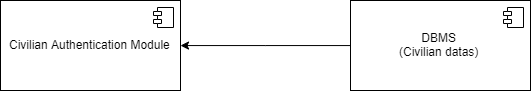
\includegraphics[width=0.85\linewidth]{Images/Integration/BasicIntegrationChart1}
		\caption{Steps 1 and 2 combined}
\end{figure}

\item \texttt{Basic Components between themselves}: and after that, this views will be integrated with their models (held in the ADSs and SafeStreets server) through a REST interface. A REST interface for receiving and sending messages will be implemented at each interacting component.The Authority's web server will be implemented offering a layer of REST communication (also the supervised learning algorithm to recognise plates) between clients and the ADS. After this, all the modules of the Basic Components groups will be up and working, as users will be able to login and report violations successfully.
\begin{figure}[H]
		\centering
			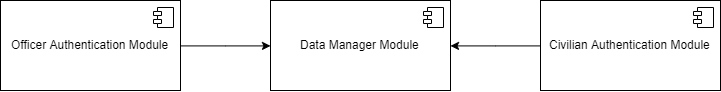
\includegraphics[width=1.0\linewidth]{Images/Integration/BasicIntegrationChart3}
		\caption{Data manager}
\end{figure}
\begin{figure}[H]
		\centering
			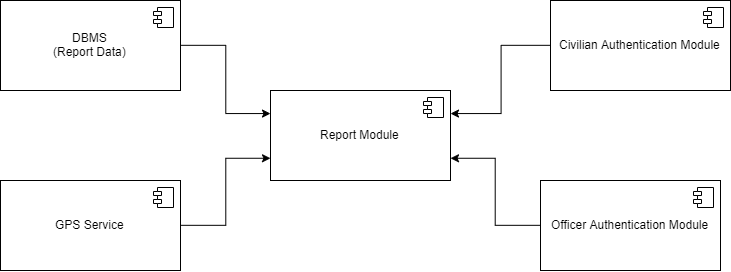
\includegraphics[width=1.0\linewidth]{Images/Integration/BasicIntegrationChart4}
		\caption{Report}
\end{figure}


\begin{figure}[H]
		\centering
			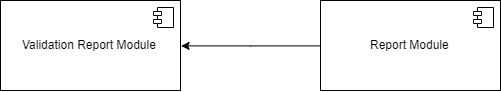
\includegraphics[width=1.0\linewidth]{Images/Integration/BasicIntegrationChart5}
		\caption{Validation report}
\end{figure}
\newpage
\item \texttt{Ticket Emission components with Basic Components}: we will start by developing the \texttt{Check Report Module} and integrating it with the \texttt{Officer Authentication Module} so that officers can successfully enter their pin when checking violations and get it authenticated.
\begin{figure}[H]
		\centering
			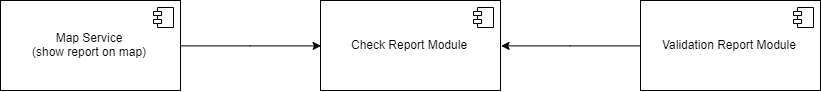
\includegraphics[width=1.0\linewidth]{Images/Integration/TicektEmissionIntegrationChart1}
		\caption{Check report}
\end{figure}
\item \texttt{Ticket Emission components with DBMS}: the \texttt{Ticket Emission Module} will be implemented and integrated with the \texttt{Check Report Module} and with the API to access both the officer accounts database (to retrieve the signature) and the one to access the data warehouse (to retrieve the correct report being written in the ticket).
\begin{figure}[H]
		\centering
			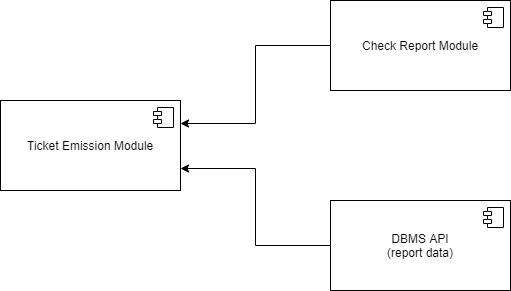
\includegraphics[width=1.0\linewidth]{Images/Integration/TicektEmissionIntegrationChart2}
		\caption{Ticket emission with check report}
\end{figure}
\newpage
\item \texttt{Ticket Emission components with Mailing Service}: to correctly send the compilated ticket to the VLA through an API.
\begin{figure}[H]
		\centering
			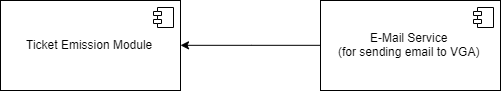
\includegraphics[width=0.8\linewidth]{Images/Integration/TicektEmissionIntegrationChart3}
		\caption{Ticket emission with email service}
\end{figure}
\item \texttt{Data Mining components with DBMS}: as the \texttt{Authority Update Module} needs to mine data from the reports data warehouse through an API.
\begin{figure}[H]
		\centering
			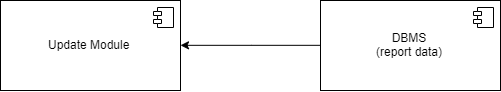
\includegraphics[width=.8\linewidth]{Images/Integration/StatisticIntegrationChart1}
		\caption{Authority Update module}
\end{figure}
\item \texttt{Data Mining components with external services}: the \texttt{Update Modules} at the client will allow unpacking and visualization of updates through the Maps services. 
\begin{figure}[H]
		\centering
			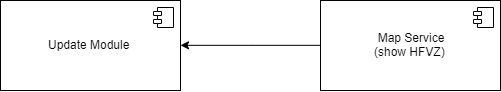
\includegraphics[width=.8\linewidth]{Images/Integration/StatisticIntegrationChart2}
		\caption{Update module}
\end{figure}
\item \texttt{Data Mining components between themselves}: the already existing REST interfaces present in all interacting components (except the SafeStreets server) will be enriched with the methods to forwards and fetch the updates.
\begin{figure}[H]
		\centering
			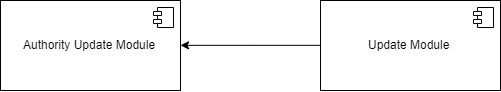
\includegraphics[width=.8\linewidth]{Images/Integration/StatisticIntegrationChart3}
		\caption{Authority update module}
\end{figure}
\end{enumerate}
\newpage
\subsection{Testing plan}
Testing will follow the order of implementation and integration described above.
Each unit of work defined in the previous section will be thoroughly tested before implementing the successive one to avoid undetected problems while integration is being performed: all the modules which have to be integrated will be tested so that their own functionalities are sure to work correctly, to ensure that if new problems arise they must be caused by the newly written code.
\\Some modules will be tested with particular attention, especially the ones regarding the Ticket Emission and Reports, to avoid wrong tickets being compiled and enforcing a certain amount of accuracy with the plate recognition, as we feel those are the most sensitive features of the application.
\newpage
\section{EFFORT SPENT}
\begin{itemize}
\item {Davide Cocco}
 \begin{center}
			\begin{tabular}{| c | l | c |}
				\hline
				\textbf{Day} & \textbf{Subject} & \textbf{Hours} \\ \hline
				14/11/2019 & High level components & 3 \\ \hline
				19/11/2019 & Component view & 4 \\ \hline
				20/11/2019 & Deployment view & 2 \\ \hline
				24/11/2019 & Sequence diagram & 5 \\ \hline
				26/11/2019 & Patterns and architectural styles & 2 \\ \hline
				26/11/2019 & Implementation, integration and testing & 4 \\ \hline
				6/12/2019 & Revision & 4 \\ \hline
				Total & & 24 \\ \hline
			\end{tabular}
		\end{center}
\item {Marco Gasperini}
\begin{center}
			\begin{tabular}{| c | l | c |}
				\hline
				\textbf{Day} & \textbf{Subject} & \textbf{Hours} \\ \hline
				14/11/2019 & Purpose and Scope & 1 \\ \hline
				19/11/2019 & Component view & 5 \\ \hline
				21/11/2019 & Requirement Traceability & 3 \\ \hline
				26/11/2019 & Implementation, integration and testing & 4 \\ \hline
				27/11/2019 & Integration charts & 3 \\ \hline
				02/12/2019 & UX diagrams & 4 \\ \hline
				6/12/2019 & Revision & 4 \\ \hline
				Total & & 24 \\ \hline
			\end{tabular}
\end{center}
\end{itemize}
\end {document}